%\documentclass[twocolumn, a4paper]{article}
\documentclass[conference]{IEEEtran}
\usepackage[utf8]{inputenc}

\newcommand\MYhyperrefoptions{bookmarks=true,bookmarksnumbered=true,
  pdfpagemode={UseOutlines},plainpages=false,pdfpagelabels=true,
  colorlinks=true,linkcolor={black},citecolor={black},urlcolor={black},
  pdftitle={pyDVS: An Extensible, Real-time Dynamic Vision Sensor Emulator using Off-the-Shelf Hardware},%<!CHANGE!
  pdfsubject={Neruomorphic vision},%<!CHANGE!
  pdfauthor={Garibaldi Pineda Garcia},%<!CHANGE!
  pdfkeywords={Computer vision, neuromorphic vision, spiking neural networks, image encoding}}%<^!CHANGE!
\ifCLASSINFOpdf
\usepackage[\MYhyperrefoptions,pdftex]{hyperref}
\else
\usepackage[\MYhyperrefoptions,breaklinks=true,dvips]{hyperref}
\usepackage{breakurl}
\fi

\usepackage{todonotes}

\usepackage[numbers]{natbib}
%\usepackage[backend=bibtex]{biblatex}
%\bibliography{biblio_dvs_emu_paper}

\usepackage{graphicx}
\graphicspath{{./pictures/}}


\usepackage{caption}
\usepackage{subcaption}
%\ifCLASSOPTIONcompsoc
%  \usepackage[caption=false,font=normalsize,labelfont=sf,textfont=sf]{subfig}
%\else
%  \usepackage[caption=false,font=footnotesize]{subfig}
%\fi

\usepackage{url}
\usepackage{amsmath}
\usepackage{amssymb}


\hyphenation{op-tical net-works semi-conduc-tor}


\begin{document}
%opening
\title{pyDVS: An Extensible, Real-time Dynamic Vision Sensor Emulator using Off-the-Shelf Hardware}
%\title{pyDVS: An Extensible, Real-time Dynamic Vision Sensor Emulator}

\author{

  \IEEEauthorblockN{Garibaldi~Pineda~García\IEEEauthorrefmark{1},~
                    Patrick~Camilleri\IEEEauthorrefmark{2},~
                    Qian~Liu\IEEEauthorrefmark{1}~and~
                    Steve~Furber\IEEEauthorrefmark{1}}
\\
  \IEEEauthorblockA{
%    \begin{tabular}{cc}
      \begin{minipage}{0.5\textwidth}
      \centering
      \IEEEauthorrefmark{1}School of Computer Science\\
      University of Manchester\\
      Manchester, United Kingdom\\
      garibaldi.pinedagarcia, qian.liu2, steve.furber\\
      @manchester.ac.uk
      \end{minipage}
      \begin{minipage}{0.5\textwidth}
      \centering
      \IEEEauthorrefmark{2}
      Entrepreneur First\\
      100 Clements Road\\
      London, United Kingdom \\
      patrick.camilleri@gmail.com
      \end{minipage}
%    \end{tabular}
  }

}


\maketitle
%\begin{multicols}{2}
%[
\begin{abstract}

Vision is one of our most important senses, a vast amount of information is perceived through our eyes. Neuroscientists have performed many studies using vision as input to their experiments. Computational neuroscientists have typically used a brightness-to-rate encoding to use images as spike-based visual sources for its natural mapping. Recently, neuromorphic Dynamic Vision Sensors (DVSs) were developed and, while they have excellent capabilities, they remain scarce and relatively expensive.


We propose a visual input system inspired by the behaviour of a DVS but using a conventional digital camera as a sensor and a PC to encode the images. By using readily-available components, we believe most scientists would have access to a realistic spiking visual input source. While our primary goal is to provide systems with a live real-time  input, we have also been successful in transcoding well established image and video databases into spike train representations. Our main contribution is a DVS emulator framework which can be extended, as we demonstrate by adding local inhibitory behaviour, adaptive thresholds and spike-timing encoding.


\end{abstract}
%]
\IEEEpeerreviewmaketitle

\section{Introduction}

In recent years the rate of increase of individual computer processors' performance has been slow; this is mainly because manufacturing technologies are reaching their physical limits. One way to improve performance is to use many processors in parallel, which has been successfully applied to parallel-friendly applications such as computer graphics. Meanwhile tasks such as pattern recognition remain difficult for computers, even with these technological advances.

Our brains are particularly good at learning and recognizing visual patterns (e.g. letters, dogs, houses, etc.). To achieve better performance for similar tasks on computers, scientists have looked to biology for inspiration. This has led to the rise of brain-like (neuromorphic) hardware, which mimics functional aspects of the nervous system. We can divide neuromorphic hardware into sensors (providing input), computing devices (which make use of information from sensors) and actuators (which control devices). Traditionally, visual input has been obtained from images that are rate-encoded, that is every pixel is interpreted as a neuron that will fire at a rate proportional to its brightness, usually via a Poisson process~\cite{snyder2012random}. While this might be a biologically-plausible encoding in the first phase of a ``visual pipeline'', it is unlikely that retinas transmit as many spikes into later stages. Furthermore, if we think in terms of digital networks, having each pixel represented by a Poisson process could incur high bandwidth requirements. 

In \citeyear{Mead1989}, \citeauthor{Mead1989} proposed a silicon retina consisting of individual photoreceptors and a resistor mesh which allowed nearby receptors to influence the output of a pixel~\cite{Mead1989}. 
Later, researchers developed frame-free Dynamic Vision Sensors (DVSs)~\cite{delbruckDVS,bernabeDVS}. These sensors feature independent pixels, which emit a signal when their log-intensity values change by a certain threshold.
These sensors have microsecond response time, excellent dynamic range properties and frame-free output, although they are (still) not as widely available as conventional cameras and are relatively expensive.

An alternative that could reduce the cost and scarcity of DVSs while keeping spike rates low is to emulate the behaviour of a DVS. \citeauthor{DVSemu} developed a DVS emulator to test behaviours for new sensor models~\cite{DVSemu}. In their work, they transform video [at 125 frames per second (FPS)] provided by a commercial camera into a spike stream. In simple terms, the emulation is done by differencing video input with a reference frame; if this difference is larger than a threshold it produces an output and updates the reference. The number of spikes produced per pixel is proportional to the difference-to-threshold ratio. This emulator has been merged into their jAER project~\cite{delbruck2008frame}, a Java-based Address-Event Representation software framework that specializes in processing DVS output in real time.

In this work, we present an extensible behavioural emulator of a DVS using a conventional digital camera as a sensor. Basing the emulator on widely available hardware allows computational neuroscientists to include video as a spike-encoded input without the cost of a DVS. We present our basic emulator in Section~\ref{sec:basic-emulator}. In Section~\ref{sec:emu-extensions} we present our extensions to the emulator. Results are given in Section~\ref{sec:results}; conclusions and suggestions for future work are given in Sections~\ref{sec:conclusions} and~\ref{sec:future-work}, respectively.


\section{The basic emulator}
\label{sec:basic-emulator}
A Dynamic Vision Sensor is a device which transforms intensity changes (in a logarithmic scale) into events. In conventional video cameras pixels capture light to form an image and repeat this process in a regular time period ($T$), these images are usually called frames (Figure~\ref{fig:dvs_vs_emu}).

\begin{figure}[htb]
  \centering
  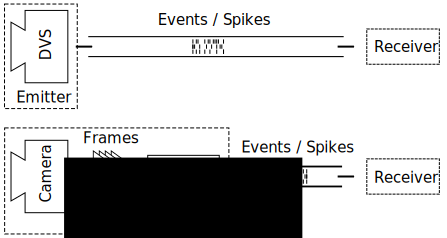
\includegraphics[width=0.4\textwidth]{dvs_vs_emu_diagram}
  \caption{DVS and emulator diagrams.}
  \label{fig:dvs_vs_emu}
\end{figure}

To emulate a frame-free system, we convert pixels' brightness differences into events. Our emulator works by analysing the difference between the latest frame captured from the camera and a reference frame. If a pixel changes by more than a certain threshold ($H$), then we generate an event which contains the pixel's coordinates and whether the change was positive or negative. 

Figure~\ref{fig:dvs_emu} shows the DVS emulation framework diagram, we obtain an image (\textsf{\footnotesize IMG}) from a video source and subtract a reference frame from it  (\textsf{\footnotesize REF}). We then apply a threshold filter to the difference frame (\textsf{\footnotesize DIFF}), the remaining pixels are considered \textit{raw spikes} (\textsf{\footnotesize SPKS}$\mathsf{_R}$). We can optionally post-process these pixels, as we'll demonstrate in Section~\ref{sec:local_inhibition}, but we must encode them so that they can be emitted as events (\textsf{\footnotesize SPKS}$\mathsf{_E}$). Finally, depending on the selected type of output encoding, we simulate a receiver and update the reference frame accordingly. 

\begin{figure}[htb]
  \centering
  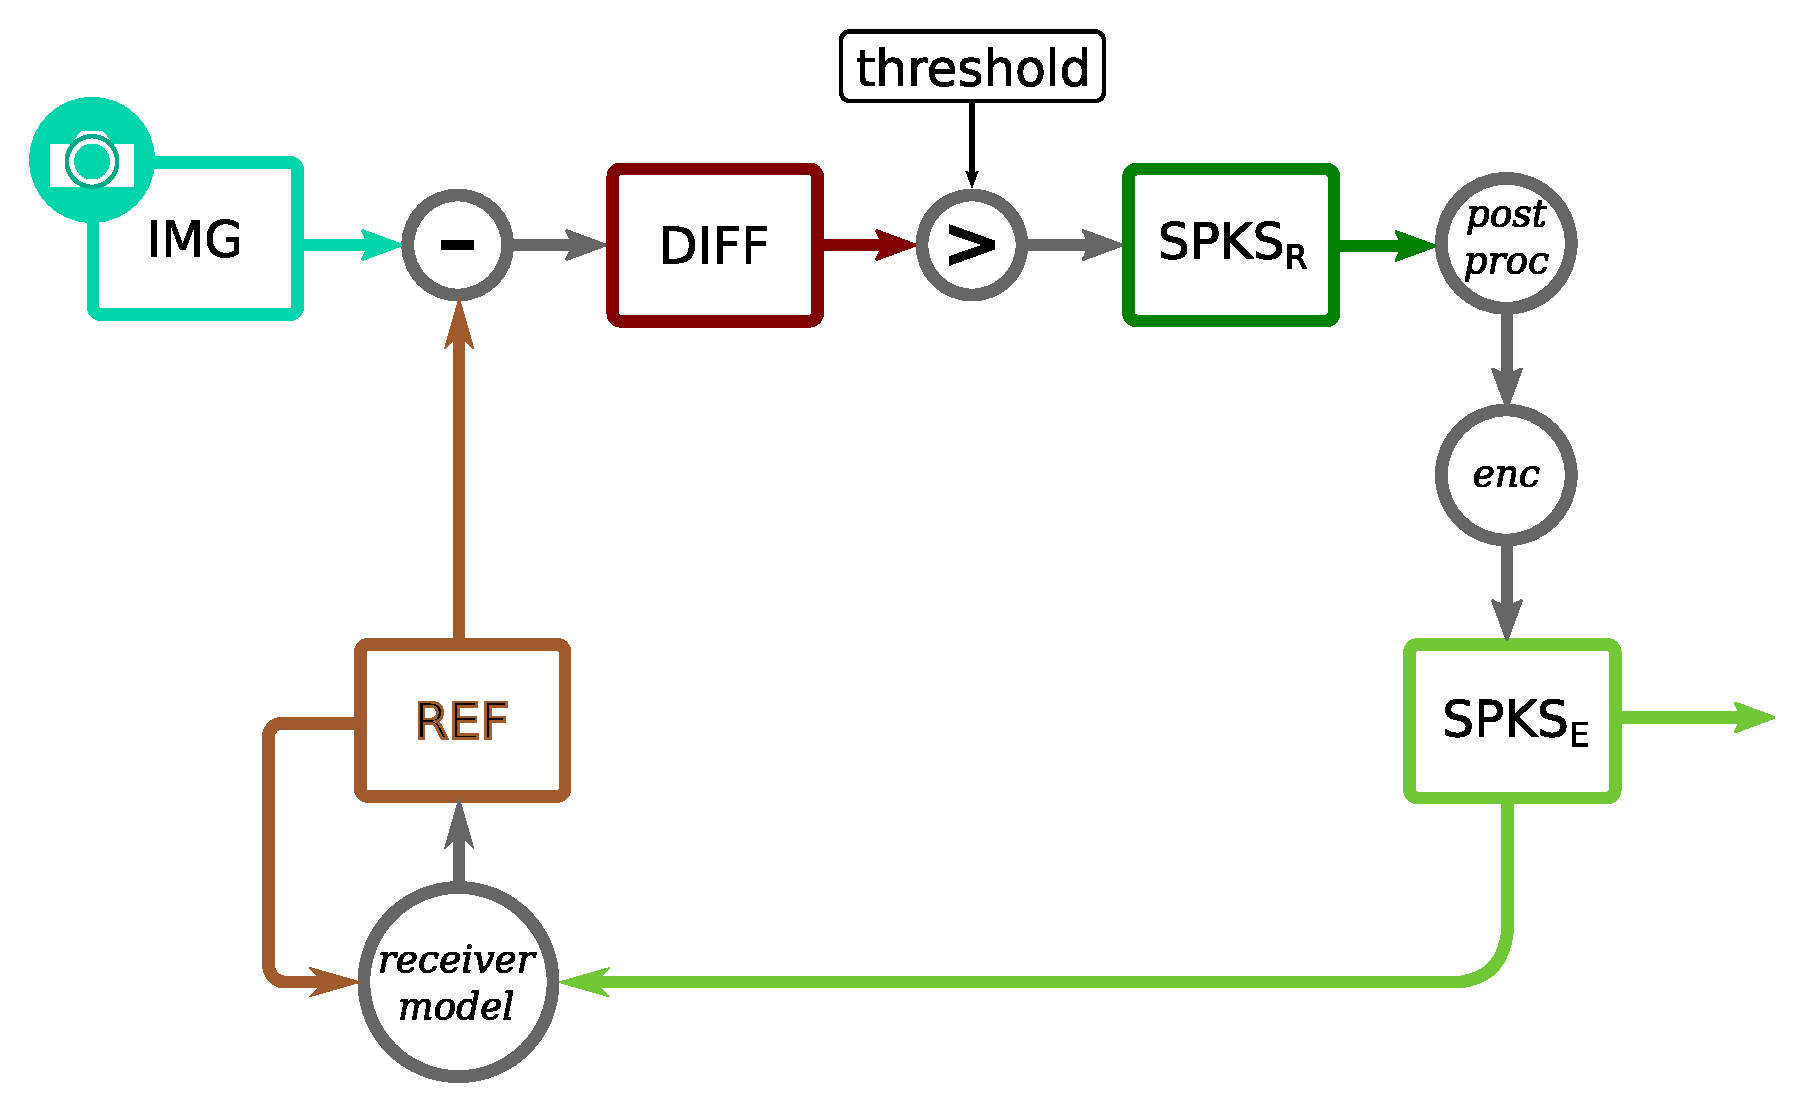
\includegraphics[width=0.5\textwidth]{dvs_emu}
  \caption{DVS emulation diagram. Circles indicate operations and rectangles stages of visual information (from frames to spike trains).}
  \label{fig:dvs_emu}
\end{figure}

Pixels in DVSs have a logarithmic response to light intensity. Similarly, most commercial cameras produce gamma-encoded images~\cite{PoyntonDigitalVideo} for better bit utilization and, in the past, to be compliant with cathode ray tube (CRT) monitors. Since this encoding's response is similar to the logarithmic one used in a real DVS (Fig.~\ref{fig:gamma_coding}), we use frame's brightness levels without modifications.
\begin{figure}[htb]
  \centering
  \includegraphics[width=0.45\textwidth]{log_vs_gamma_response}
  \caption{Logarithmic and Gamma response functions (normalized, $\gamma = 2.2$)}
  \label{fig:gamma_coding}
\end{figure}
% Figure~\ref{fig:gamma_coding} shows the response for the encoding process (crosses), CRT monitors (hexagons) and decoding process (dots). 



We have constrained the output of our system to emit events in discrete time, so we divide time period $T$ into $N_{b}$ bins of width $t_{b}$ (Fig.~\ref{fig:time_bins}), and neurons (representing pixels) are only allowed to spike once per time bin. For example, if time interval $T = 10 ms$ and $N_{b} = 10$ then $t_{b} = 1 ms$, so neurons would fire at most once per millisecond. Since we are developing a real-time system, all events should be emitted between frames, so the maximum number of spikes per neuron per frame is $N_{b}$.

\begin{figure}[hbt]
  \centering
  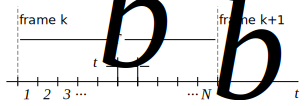
\includegraphics[width=0.4\textwidth]{discrete_time_bins}
  \caption{Time discretization.}
  \label{fig:time_bins}
\end{figure}

As in previous emulators~\cite{DVSemu}, our basic emulator's output format is rate-based. Each emitted spike signifies the pixel changed by $H$ brightness levels, where $H$ is also the threshold. Let $N_{H}$ be the integer division of a pixel's brightness change $\Delta B$ by the threshold $H$ and limiting by $N_{b}$, the number of spikes ($N_{s}$) needed to represent $\Delta B$ will be
\begin{equation}
  \label{eq:num_spikes_rate}
  N_{s} = \mathrm{min}\left( N_{b}, \;\; N_{H} \right) 
        = \mathrm{min}\left( N_{b}, \;\; \left\lfloor\frac{\Delta B}{H}\right\rfloor \right)
\end{equation}
At this stage we model a perfect receiver, so the update rule for the reference is
\begin{equation}
  \label{eq:ref_update}
  R_{now} = R_{last} + N_{s}\cdot H
\end{equation}


\section{Emulator extensions}
\label{sec:emu-extensions}
In its worst case rate-based encoding can send a spike per millisecond per pixel each frame, which is not biologically plausible and can potentially saturate communication channels. 
%If we think of a camera which captures images with a $128\times 128$ resolution at 30~FPS, it can generate up to about 5K Spikes/sec. This translates to, approximately, 10Mbit/sec (without transmission packet's header data).
Two of the extensions we have developed diminish the rate of spikes, either by changing output encoding~(Sec.~\ref{sec:output-modes}) or post-processing generated spikes~(Sec.~\ref{sec:local_inhibition}). 

Another extension adds robustness to transmission by adding a history decay mechanism~(Sec.~\ref{sec:hist_decay}). The final extension replaces the constant threshold for an adaptive version (Sec.~\ref{sec:adaptive_thresh}). Figure~\ref{fig:dvs_emu_inh} shows modifications on the basic DVS emulator.  
\begin{figure}[htb]
  
  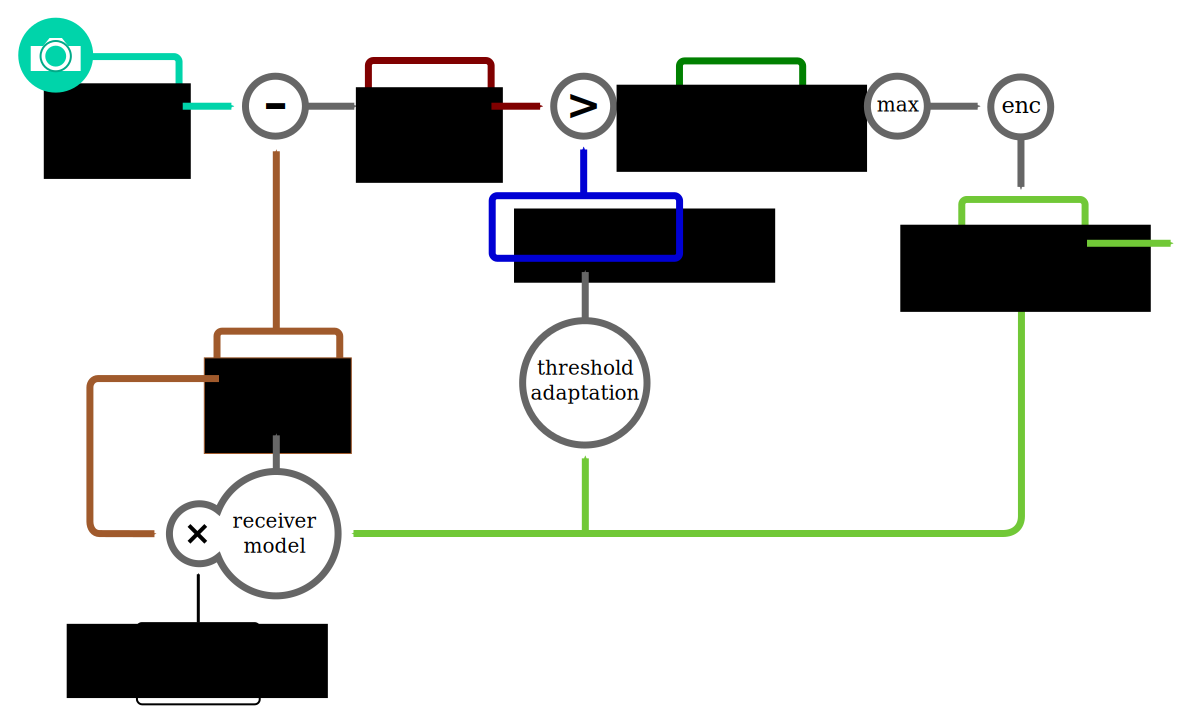
\includegraphics[width=0.5\textwidth]{dvs_emu_decay_adapt_inh}
  \caption{DVS emulation with adaptive thresholds, local inhibition and history decay.}
  \label{fig:dvs_emu_inh}
\end{figure}


\subsection{Spike-time encoding}
\label{sec:output-modes}

One way to prevent high spike rates is to encode the brightness difference in the time a spike is emitted, similar to how pulse-position modulation works~\cite{book:ppm}. That is each time bin represents a brightness change, in either a linear or logarithmic scale. Furthermore, there's evidence that neurons use spike timing to encode values~\cite{Singer1999189} and some theories of neural computation require spike-time coding~\cite{izhikevich2006polychronization}. 


\begin{figure}[hbt]
  \captionsetup[subfigure]{justification=centering}
  \begin{center}
    \begin{subfigure}[b]{0.25\textwidth}
      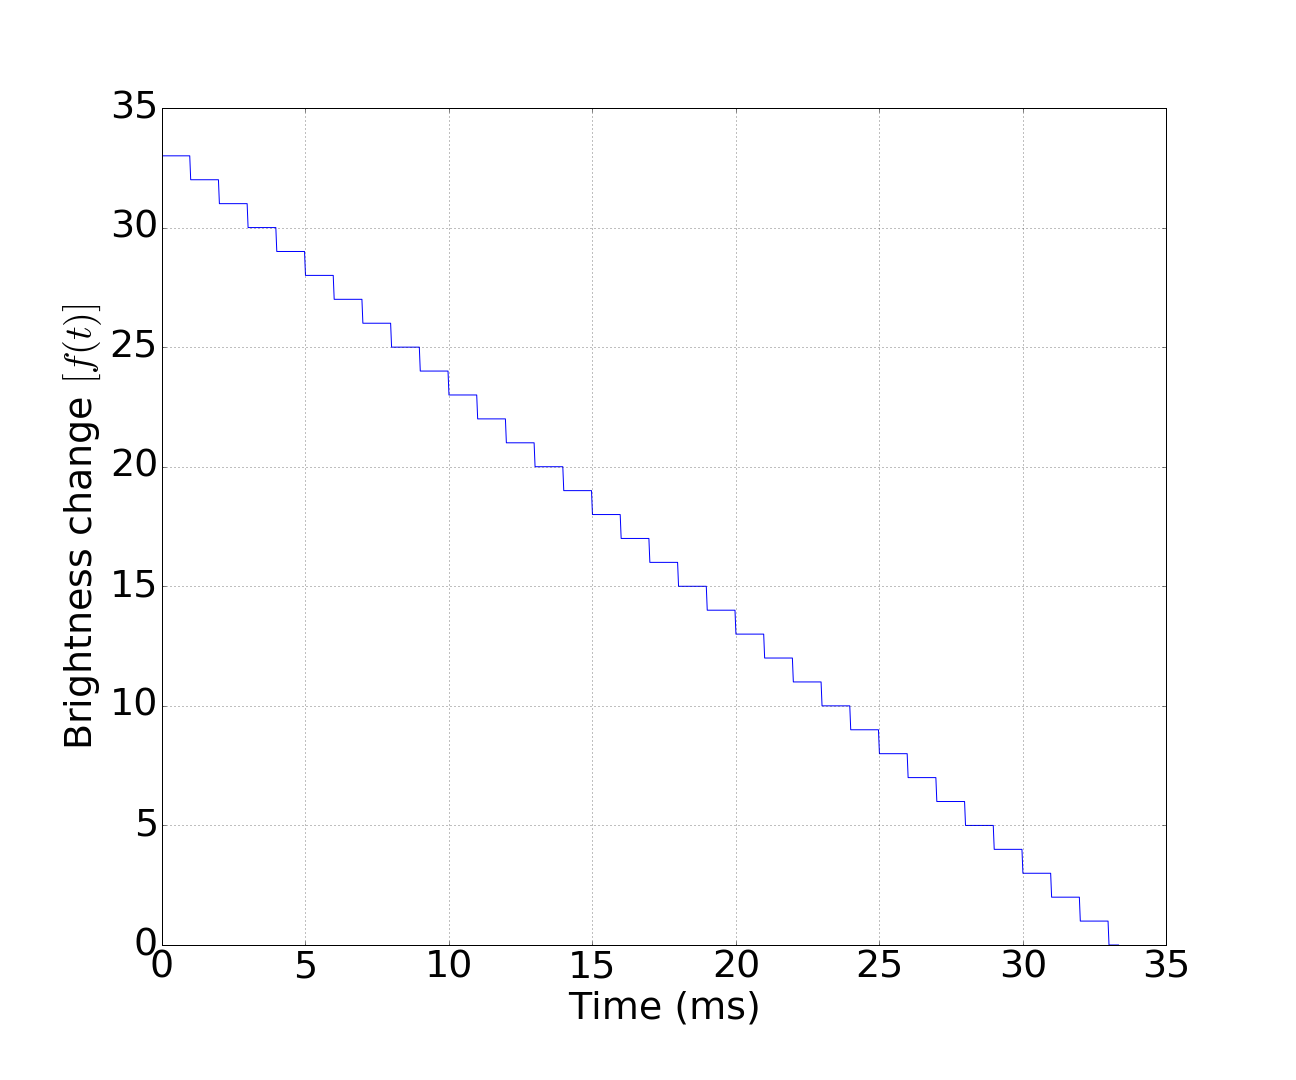
\includegraphics[width=\textwidth]{linear_response_graph}
      \caption{Linear response \\($N_{b}=33$, $t_{b}=1.1$).}
      \label{fig:linear_time_resp}
    \end{subfigure}~
    \begin{subfigure}[b]{0.25\textwidth}
      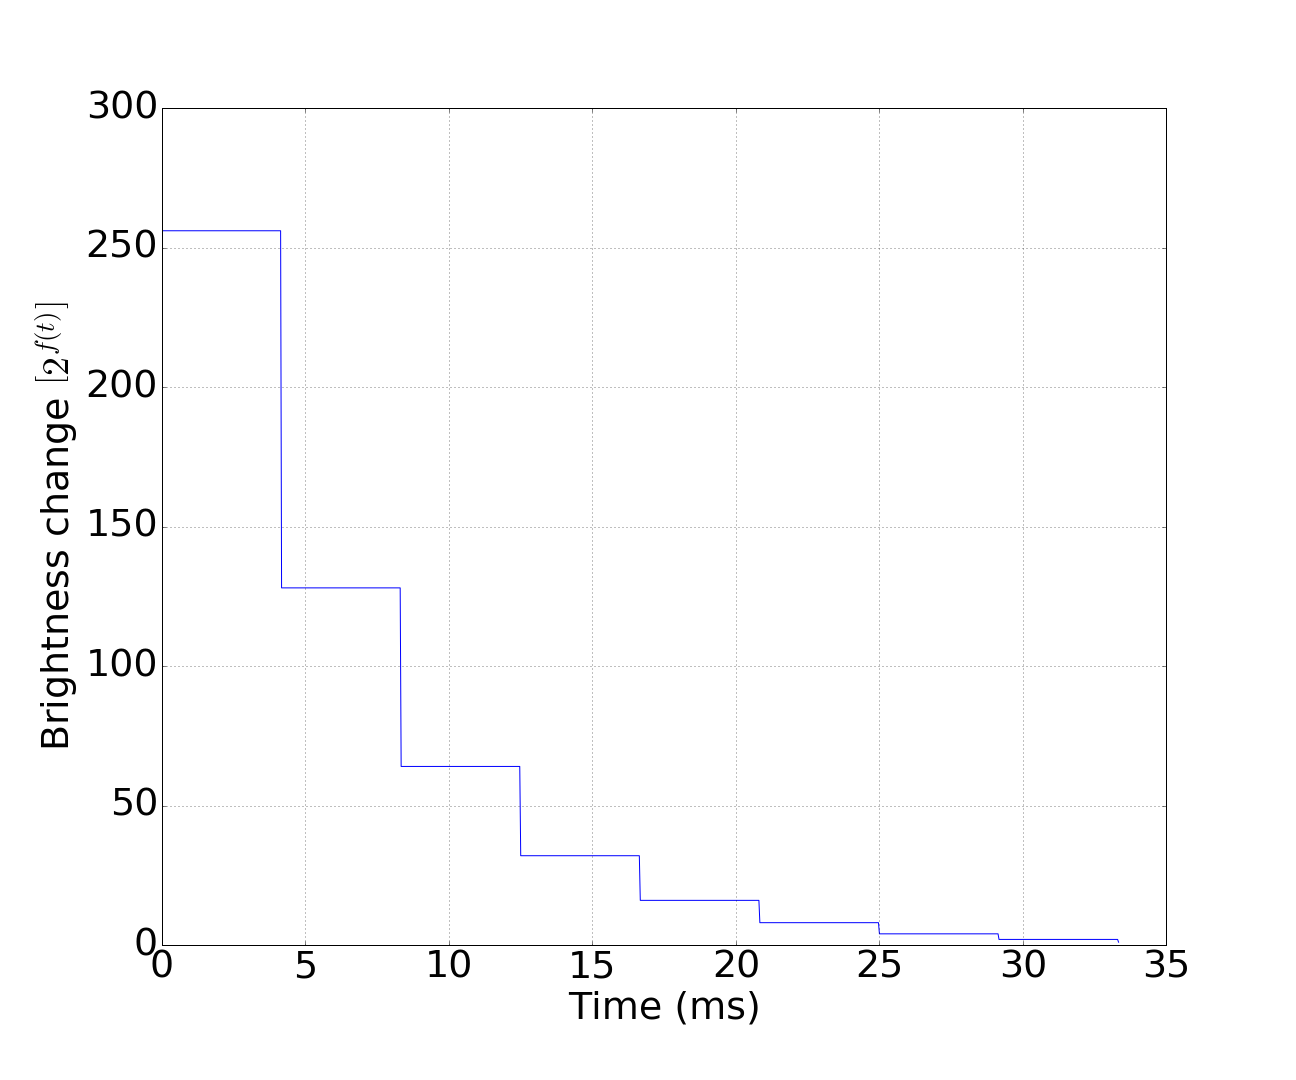
\includegraphics[width=\textwidth]{logarithmic_response_graph}
      \caption{Logarithmic response\\($N_{b}=8$, $t_{b}=4.16ms$).}
      \label{fig:logaritmic_time_resp}
    \end{subfigure}
    
    \caption{Possible values for a spike timing code, linear (left) and logarithmic (right) scales $\left(FPS = 30, T=33.3 ms\right)$.}
    \label{fig:linear_log_response}
  \end{center}
\end{figure}

Since brightness variations happen when a new frame is captured, spike times are referenced to the beginning of each frame. To synchronize the emitter with the receiver, we send one spike for each pixel at the beginning of the simulation $(t=0)$ and all of these encode a predefined value (in this case the maximum one). Figure~\ref{fig:linear_log_response} shows a single frame, spikes that were sent closer to the frame's beginning encode larger values. This means that if spikes were emitted at $t_{0}$ and $t_{1}$,  then a pixel changed $X$ and  $Y$ times the threshold, respectively. In our system, if $t_{0} < t_{1}$ then $X > Y$.

We will first present the linear scale case, we can calculate the appropriate time bin $C_{b}$ with
\begin{equation}
\label{eq:linear_bin_calc}
C_{b} = N_{b} - \mathrm{min}\left( N_{b}, \;\; N_{H} \right),
\end{equation}
and the time at which the spike will be sent is given by
\begin{equation}
t_{s} = C_{b}t_{b}
\end{equation}

The main advantage of this encoding is that a single spike could represent multiple (at most $N_{b}$) rate-based spikes, though the encoded values are limited by time resolution and the frame rate of the camera.

If a receiver wants to decode the spikes, it needs to figure out the time at which each frame begins, but we do not provide information about this event. A possible solution involves keeping track of the time and value from the last collected spike, by keeping these values we can calculate the end of the previous spike's frame. The green line in Figure~\ref{fig:linear_time_all} shows this spike time-to-value relation. 

\begin{figure}[htb]
  
  \centering
  
  \begin{subfigure}[b]{0.45\textwidth}
    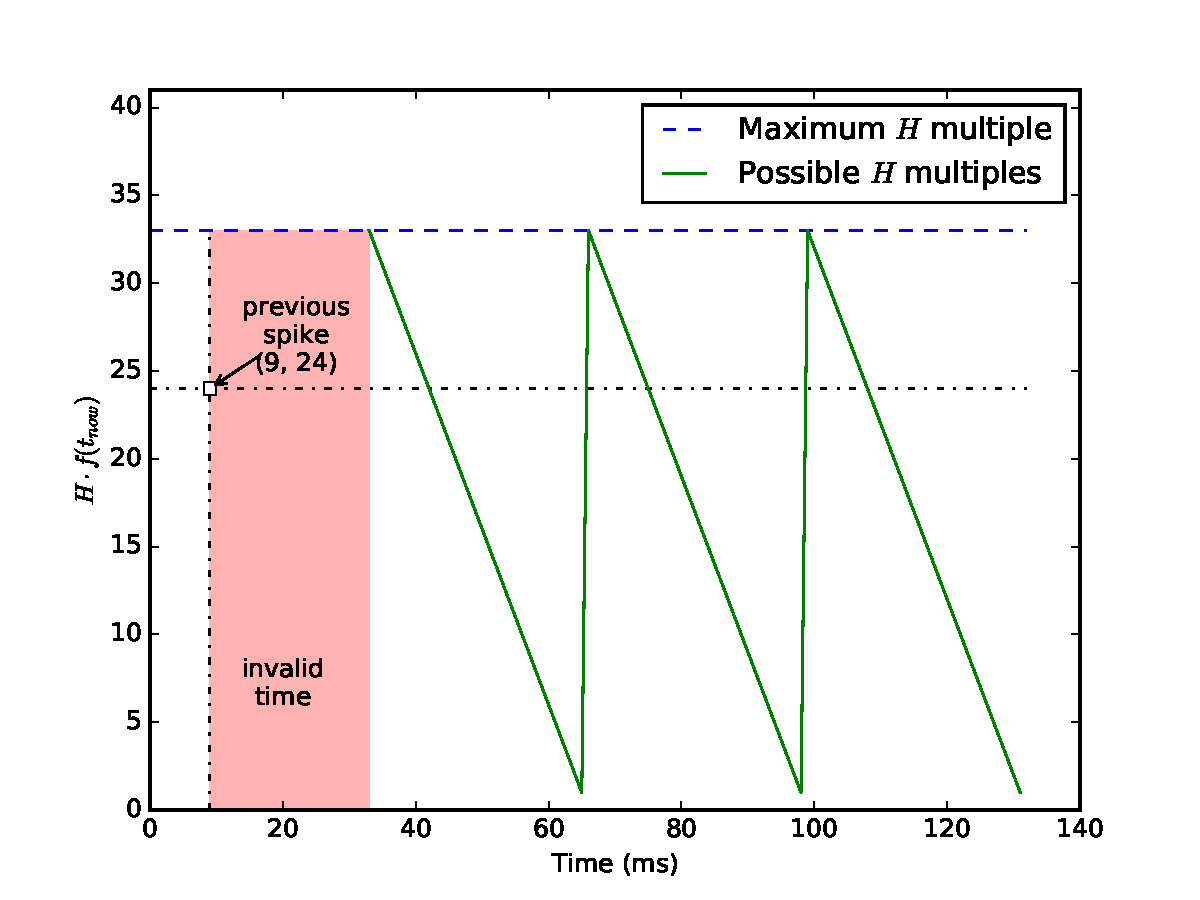
\includegraphics[width=\textwidth]{spike_values_linear}
    \caption{Possible values for spikes received after another.}
    \label{fig:linear_time_all}
  \end{subfigure}
  
  \begin{subfigure}[b]{0.45\textwidth}
    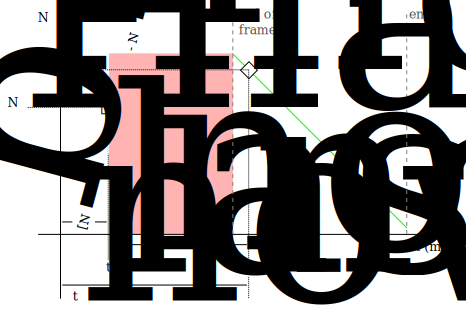
\includegraphics[width=\textwidth]{new_val_calc_linear}
    \caption{Time differences between current and previous spikes.}
    \label{fig:linear_time_calc}
  \end{subfigure}
  \caption{Spike-time coding. Decoding values in linear scale $(FPS=30,T=33.3ms)$.}
  \label{fig:linear_time}
\end{figure} 


Let $\Delta t$ be the difference in arrival time between the current spike and the end of the previous spike's frame (Fig.~\ref{fig:linear_time_calc}, center). To calculate it we use
\begin{equation}
\Delta t = t_{now} -  \left(t_{last} + N_{H}^{last}t_{b}\right)
\label{eq:time_diff}
\end{equation}
where $N_{H}^{last}W_{b}$ shifts $t_{last}$ to the end of its frame. By having $\Delta t$ anchored at the beginning of a frame we can compute its bin with the remainder of the division with time period $T$.

\begin{equation}
C^{now}_{b} = \frac{ \mathrm{mod}\left(\Delta t, \;\; T\right) }{ t_{b} }
\label{eq:bin_compute}
\end{equation}
here, `$\mathrm{mod}$' calculates its arguments division remainder. Now that the time bin $C_{b}$ is known we can compute the brightness difference with
\begin{equation}
 \Delta B = H\cdot N_{H}^{now} =  H\left(N_{b} - C^{now}_{b}\right) 
 \label{eq:new_Nh_linear}
\end{equation}

%and reduce the probability of getting the wrong value
We've mentioned before that the maximum brightness difference in linear scale is $N_{b}\cdot H$, by using a logarithmic scale we can encode larger brightness differences and even do so with wider time bins. This also reduces the chances of wrongly decoding spikes. If the maximum brightness difference possible is 255 and the threshold is 12, we only need 5 time bins to express the largest change. 
%Since we are using a single spike, the value encoded in spike timing will be an approximate one. 
The time bin can be calculated with Equation~\ref{eq:log_bin_calc}. Figure~\ref{fig:exponential_time} shows the relation of spike time and brightness change with logarithmic scale.
\begin{equation}
\label{eq:log_bin_calc}
C_{b} = N_{b} - \mathrm{min}\left( N_{b}, \;\; \lfloor\log_{2} N_{H}\rfloor \right) 
\end{equation}

The time at which the spike would be sent, with respect to the beginning of the frame would be $t_{s} = C_{b}t_{b}$.
%The main advantage of this technique would be to achieve large values with fewer time bins as the growth is exponential (Fig. \ref{fig:exponential_time}). We propose to use this encoding in two ways: \textit{shoot-and-refine} and \textit{full value}. 
Since a single spike per pixel per frame is emitted, we are sending an underestimate of the desired value (i.e. previous power of two). In the following frames we send spikes to refine the received value towards the desired one~\cite{sardac}. 

\begin{figure}[htb]
  \centering
  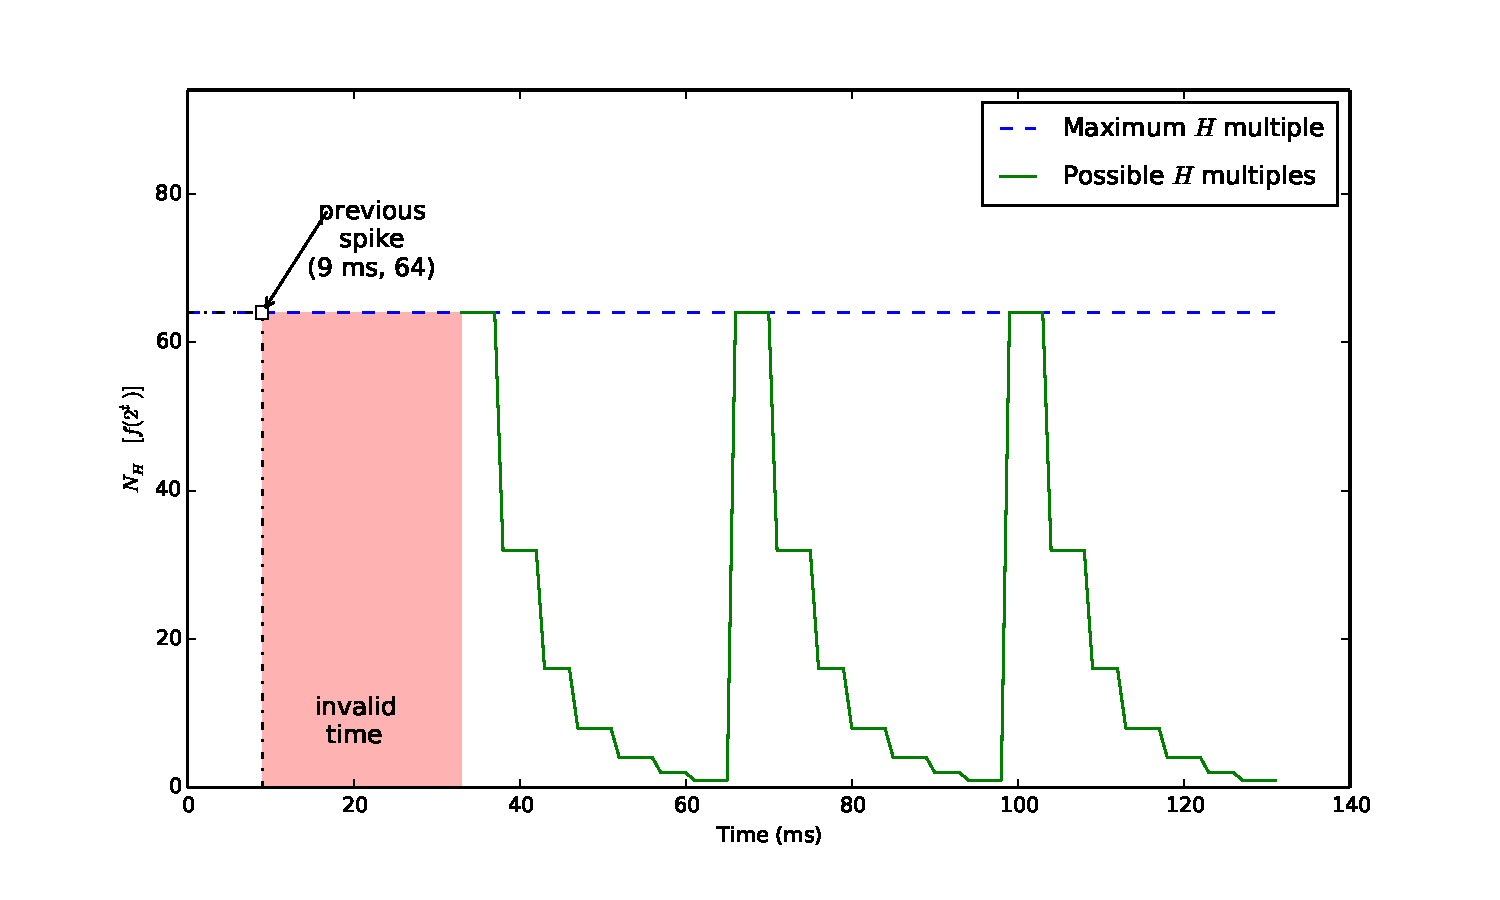
\includegraphics[width=0.45\textwidth]{spike_values_exp}
  
  \caption{Spike-time coding. Decoding values in logarithmic scale. Frame rate was 30 FPS and we used 7 bits (time bins). }
  \label{fig:exponential_time}
\end{figure} 

Decoding (Fig.~\ref{fig:exponential_time}) can be done in a similar way to the linear case, but the receiver can only record an approximate version of $N_{H}$, that is $\tilde{N}_{h} = 2^{\lfloor\log_2 N_{H}\rfloor}$. The time difference with respect to the end of frame for the previous spike is
\begin{equation}
\Delta t = t_{now} - \left( t_{last} + \log_{2}\tilde{N}_{H}t_{b} \right)
\label{eq:time_diff_exp}
\end{equation}

The current spike's time bin is calculated using Eq.~\ref{eq:bin_compute} and the decoded value with
\begin{equation}
\Delta B = H\cdot N_{H}^{now} = H\cdot 2^{ \left( N_{b} - \lfloor C^{now}_{b}\rfloor  \right)}
\label{eq:new_Nh_exp}
\end{equation}

If we allow many spikes to be sent per pixel per frame, the receiver gets a closer approximation of $N_{H}$. The downside to this is that this is unlikely to be biologically plausible. Decoding multiple spikes per frame has to be split in two cases: first, if the new spike arrives before the current frame period is finished, then we accumulate its value to the current decoded value; otherwise we keep the newly decoded value. 

%\setcounter{figure}{9} % -------------- fix figure numbers ----------------- %

%\subsection{Additional behaviours}

%\subsubsection{History decay} % - What if spikes get lost?}
\subsection{History decay} % - What if spikes get lost?}
\label{sec:hist_decay}
Initially we described a system where we assume every spike sent will be captured and properly decoded by the receiver, but this is not always the case. To cope with failures in transmission, we now introduce a history decay mechanism which will allow the receiver to, in the long term, recover from missing spikes. Let $D \in \mathbb{R} = (0, 1]$ be the weight for the reference frame in the calculation of its new value, the update rule becomes
\begin{equation}
\label{eq:ref_update_decay}
R_{now} = D\cdot R_{last} + N_{H}\cdot H
\end{equation}
If no spikes are sent, the values in the reference frame tend to 0 which corresponds to black in our tonal scale. This can be seen as ``forgetting'' the information stored in the reference frame.
%\begin{figure}[htb]
%  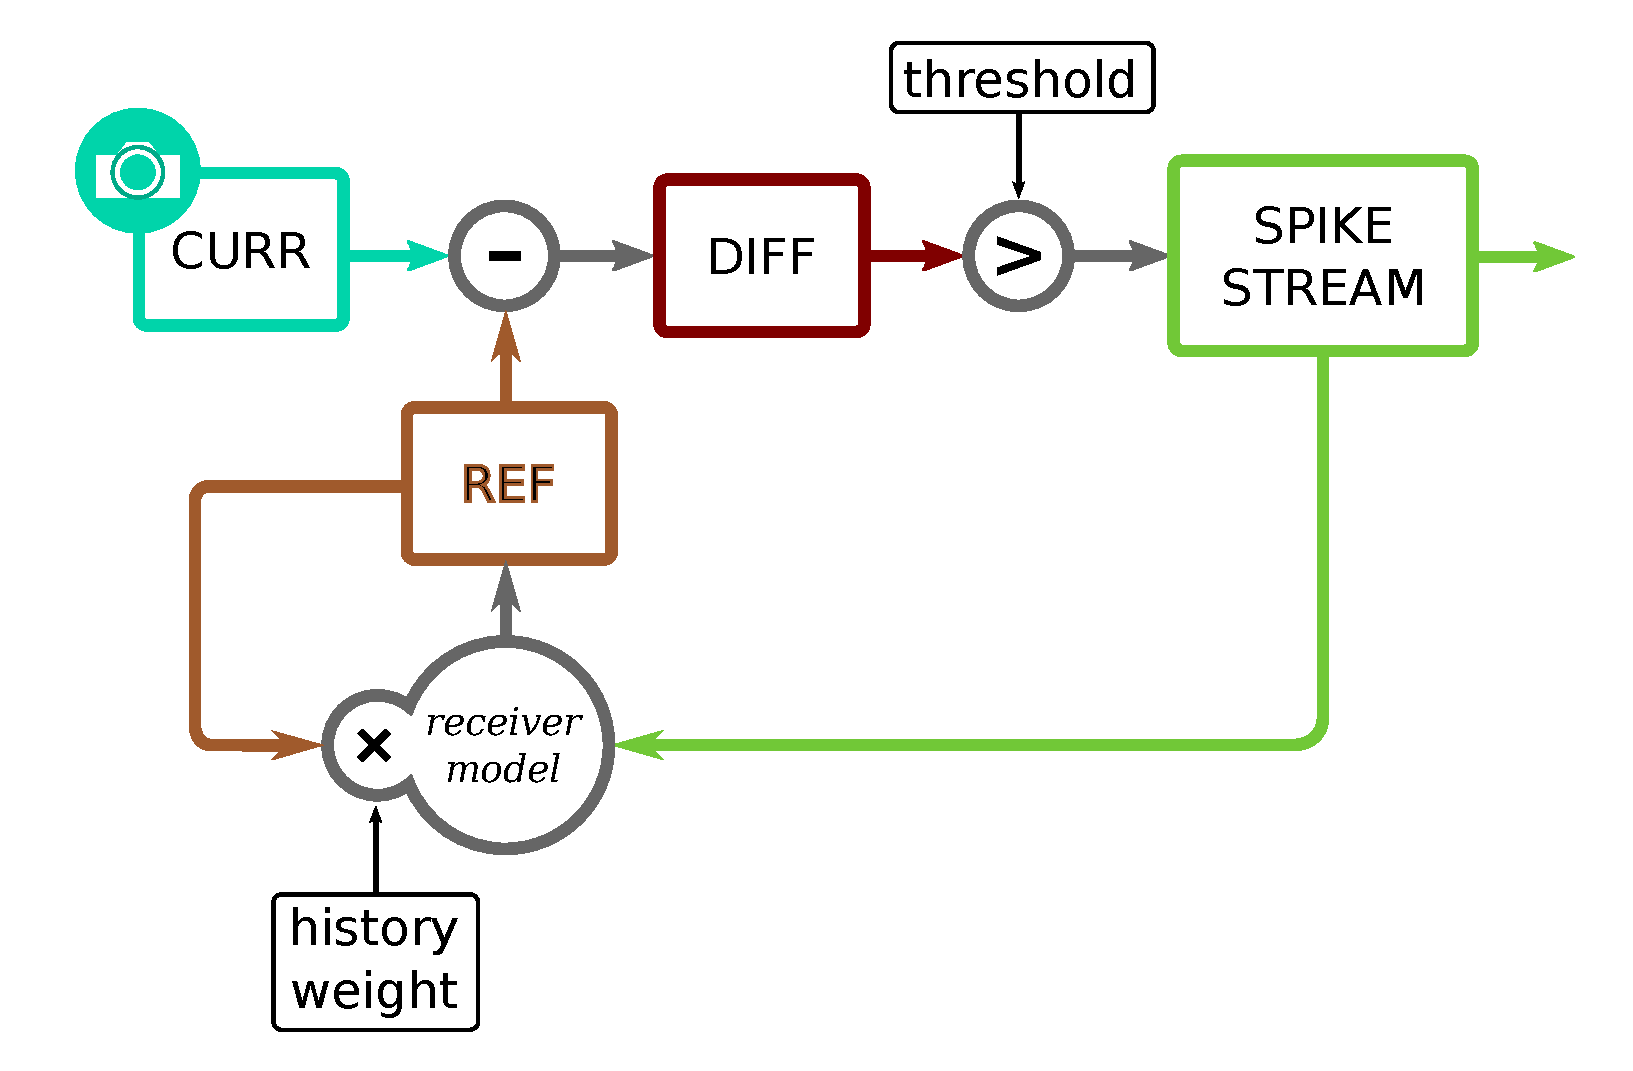
\includegraphics[width=0.5\textwidth]{dvs_emu_decay}
%
%  \caption{DVS emulation with history decay.}
%%  \label{fig:dvs_emu_decay}
%\end{figure}

%\subsubsection{Adaptive threshold} 
\subsection{Adaptive threshold}
\label{sec:adaptive_thresh}
Slow-changing pixels in cameras would capture small brightness values each frame thus the difference would never be enough to generate a spike. Meanwhile DVSs' pixels receiving insufficient light to immediately trigger a spike, still gain some charge and, after some time, will generate a spike event. We propose to mimic this behaviour by adapting the threshold on a per-pixel basis, so we reduce the threshold if a pixel did not emit a spike. Since threshold values may be lowered, they also have to be increased if a spike was generated. These changes in the threshold effectively add a temporal low-pass filter to the system. 

%\begin{figure}[htb]
%
%  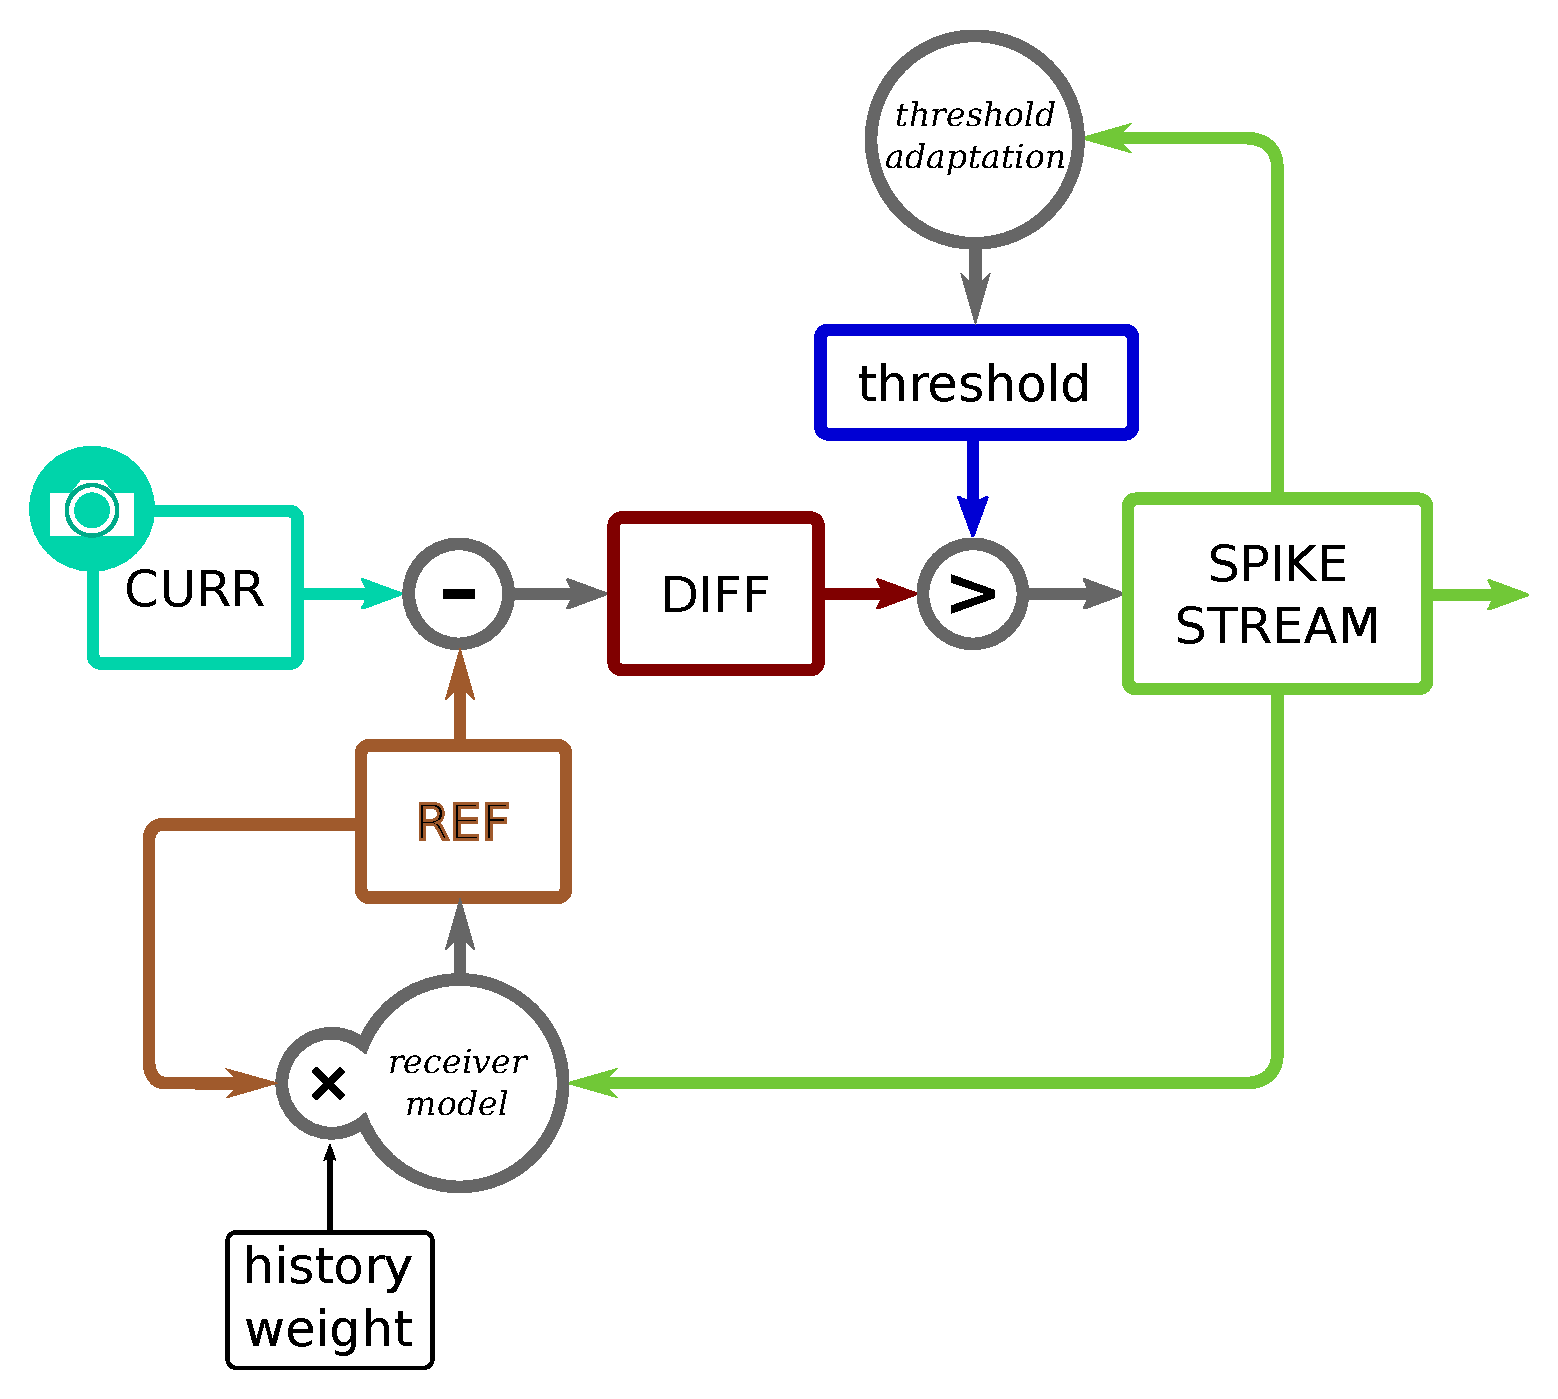
\includegraphics[width=0.5\textwidth]{dvs_emu_decay_adapt}
%  \caption{DVS emulation with adaptive thresholds.}
%  \label{fig:dvs_emu_adapt}
%\end{figure}
%\setcounter{figure}{8} % -------------- fix figure numbers ----------------- %
\begin{figure}[hbt]
  \centering
  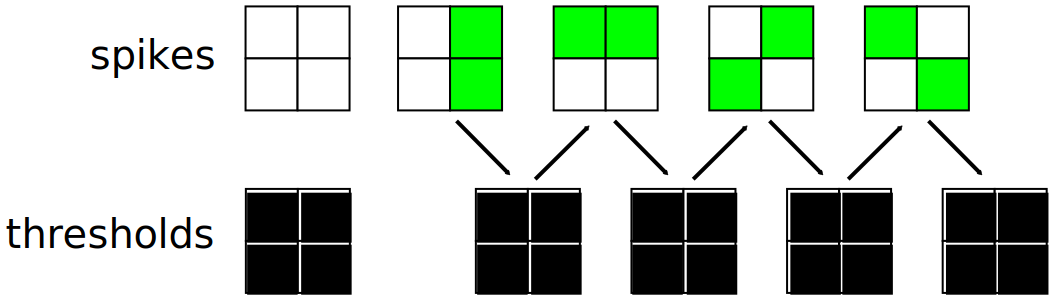
\includegraphics[width=0.45\textwidth]{adaptive_thresh_boxes}
  \caption{Adaptive threshold behaviour.}
  \label{fig:adpt_thresh}
\end{figure}

%\subsubsection{Local inhibition} 
\subsection{Local inhibition}
\label{sec:local_inhibition}
In mammalian retinas inhibitory circuits play an important role. Some researchers have suggested that they reduce the number of spikes needed to represent what the eye is sensing~\cite{basab}. Our emulator's inhibition mechanism follows a similar idea; since neighbouring pixels have similar values, we assume that they are transmitting redundant information. The inhibitory behaviour is simply a local MAX operation (similar to complex cells in the HMAX model~\cite{riesenhuber1999hierarchical}) of pixel areas. An example is shown in Figure~\ref{fig:local_inh}, we chose a 2-by-2 area since it's the smallest 2D one. Initially pixels whose difference was 77, 31, -16 (left side in green and red) where to emit events, but after inhibition only the maximum value (right side in green; 77) will generate a spike, while other values (right side in brown; 0, 31, and 16) are blocked.

%\setcounter{figure}{10} % -------------- fix figure numbers ----------------- %
\begin{figure}[htb]
\centering
    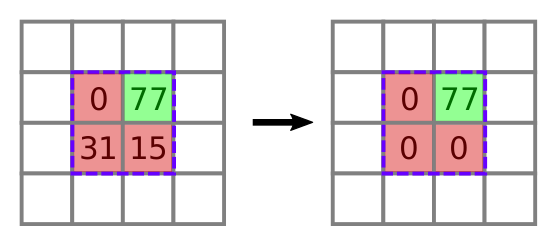
\includegraphics[width=0.3\textwidth]{inh_local_max_img}
    \caption{Local inhibition mechanism. Quantities represent the absolute value of the difference between an image and the reference. Green and red mean a spike event, brown pixels did not spike}

  \label{fig:local_inh}
\end{figure}

\section{Results}
\label{sec:results}
The emulator was developed and tested in a desktop computer (Intel i5, 8GB RAM) using the Python and Cython programming languages. We targeted a maximum $128\times 128$-pixel resolution, which can perform at a 60 FPS [lower resolutions (64, 32 and 16 pixel) are also available and can run at higher frame rates]. This project is open source and is available at \url{https://github.com/chanokin/pyDVS}.

The initial goal was to provide an alternative for computational neuroscientists who required spiking visual input but could not afford a DVS. To test the emulator compatibility with neuromorphic hardware, we created a PyNN-compatible~\cite{pynn} code template that communicates to the SpiNNaker platform~\cite{spinnakerOverview} over Ethernet. We tested the behaviour of a DVS~\cite{bernabeDVS} and our emulator with a PS3Eye camera~\cite{wikipedia:ps3eye}. Figure~\ref{fig:dvs_vs_cam} shows a visual comparison of the behaviour of the emulator (left) and the DVS (right); the emulator's output has some noise due to automatic mechanisms (e.g. exposure, gain control, white balance). Since these have low difference values, they could be filtered out by changing the threshold.


\begin{figure}[htb]
  \captionsetup[subfigure]{justification=centering}
  
  \centering
  \begin{subfigure}[b]{0.21\textwidth}
    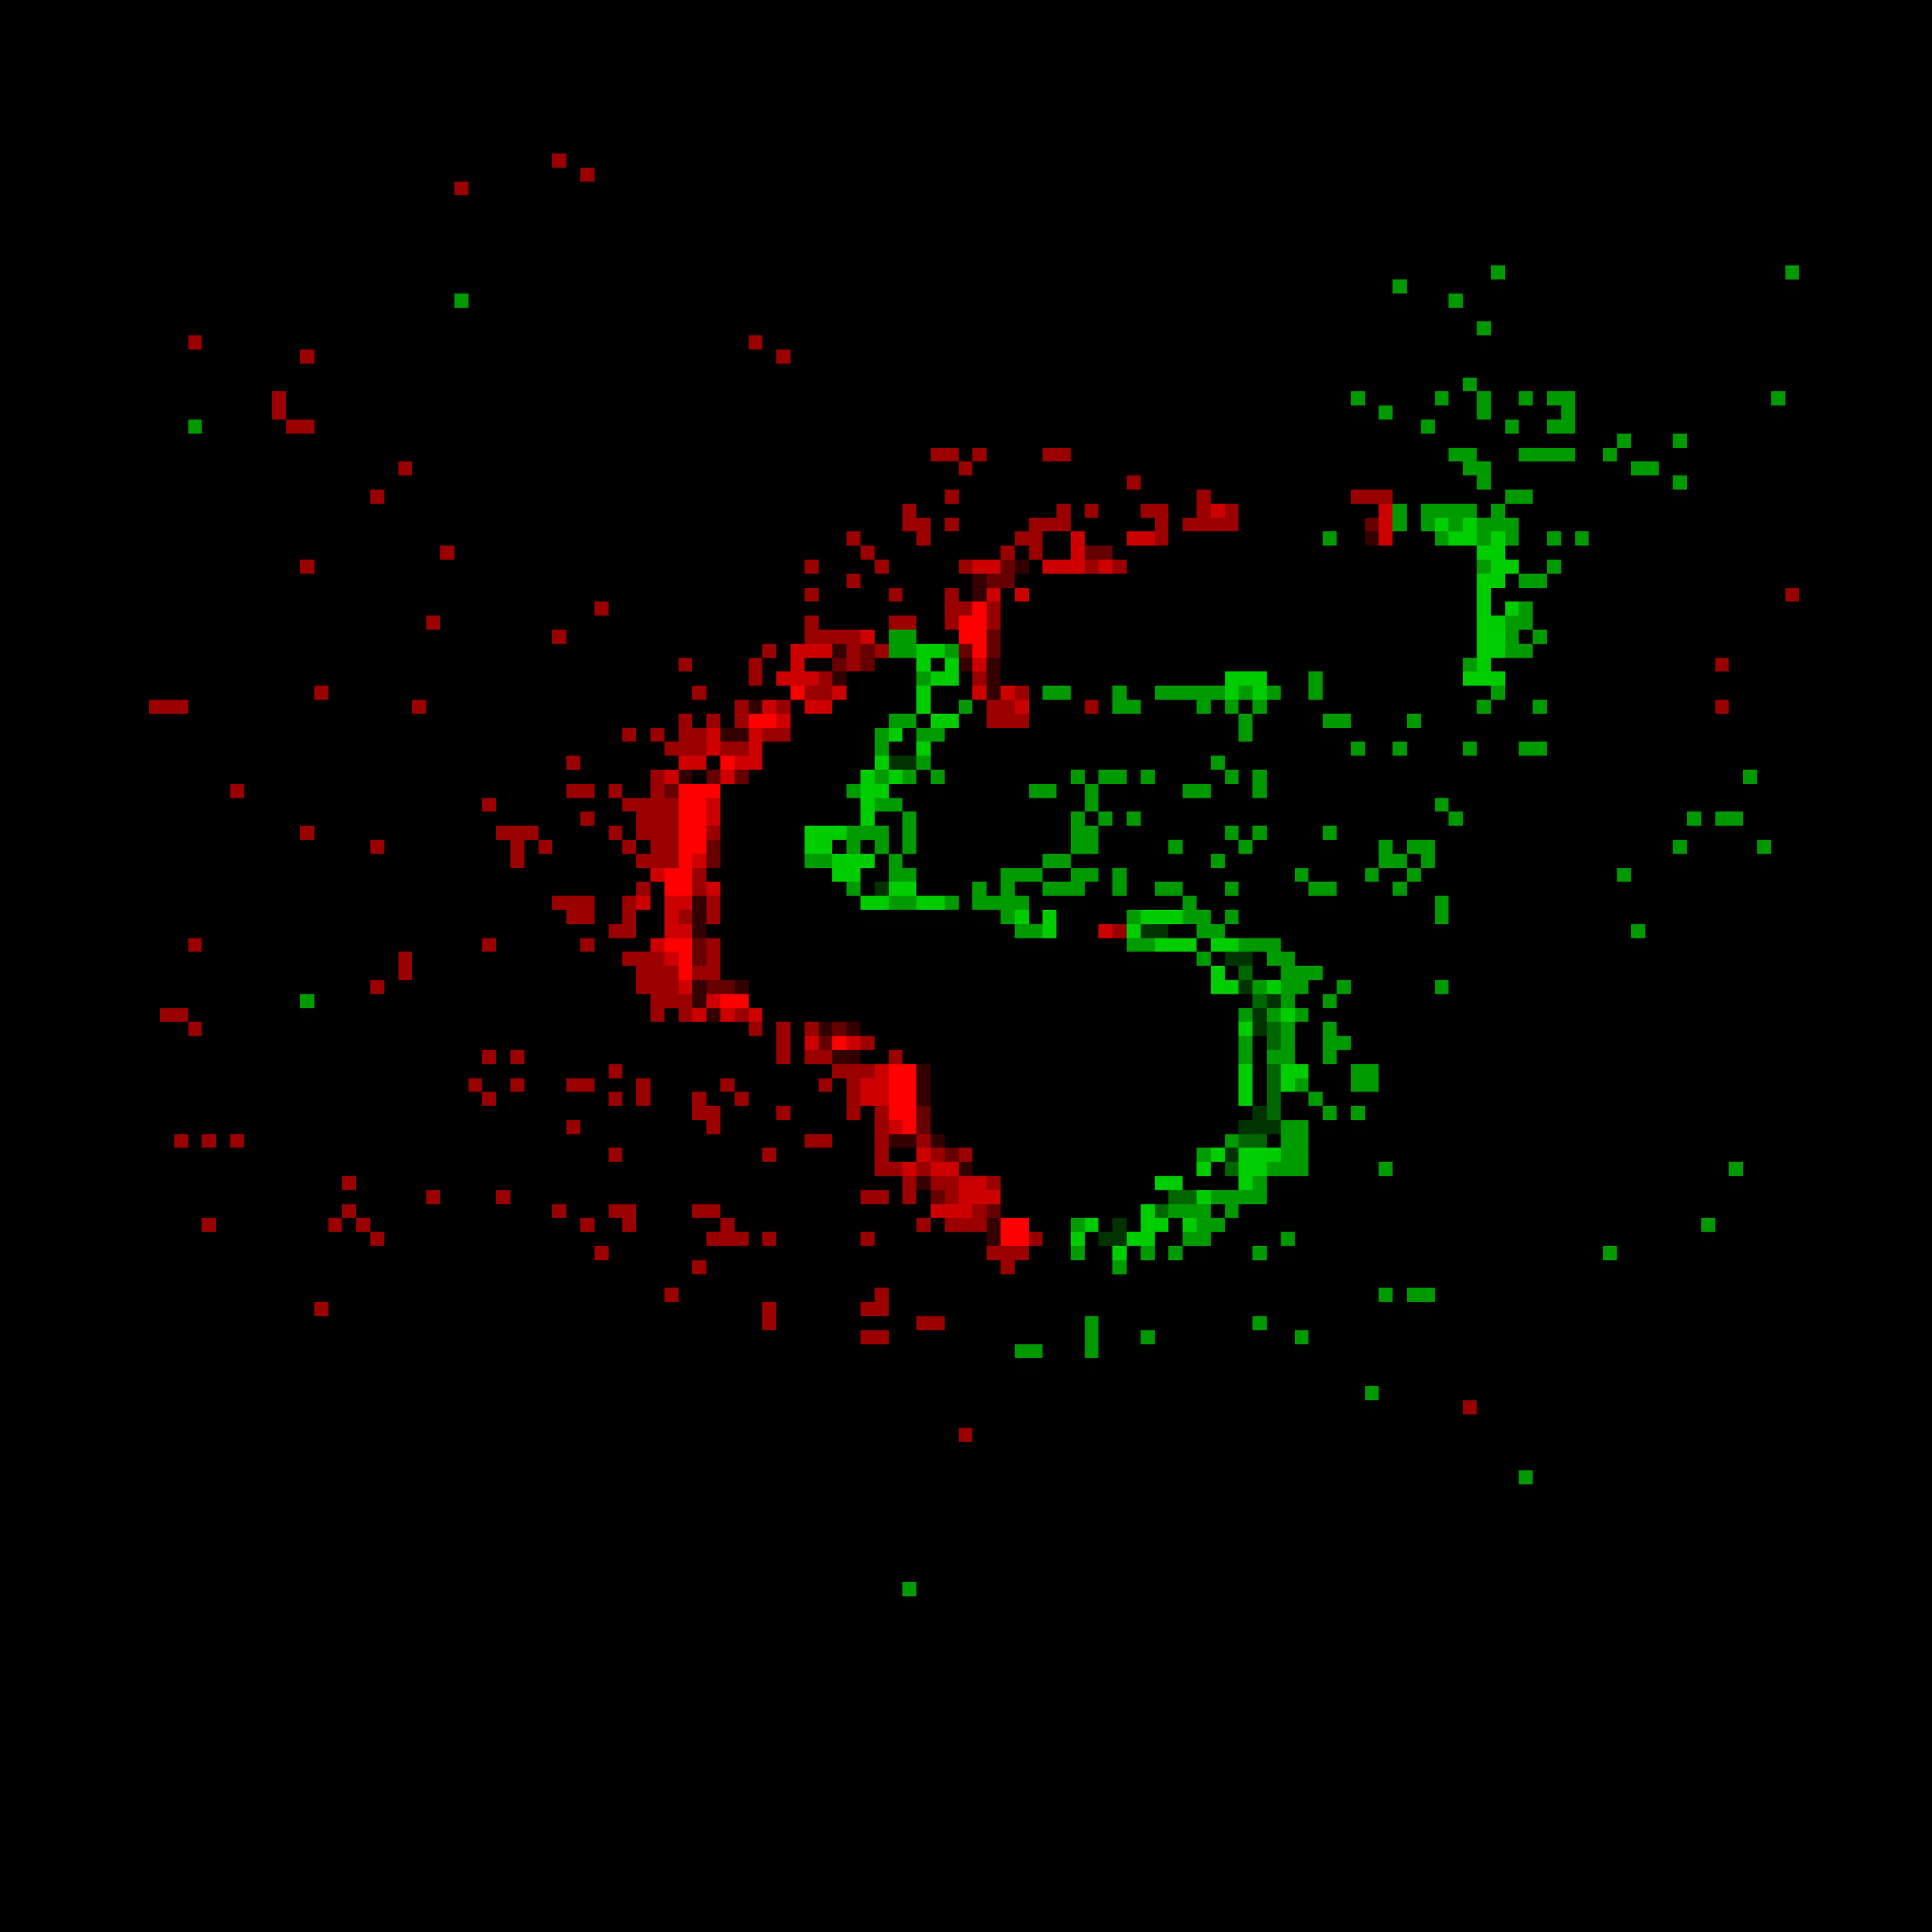
\includegraphics[width=\textwidth]{camera_demo_1}
    \caption{Recording from \\DVS emulator. }
    \label{fig:cam_demo}
  \end{subfigure}~
  \begin{subfigure}[b]{0.21\textwidth}
    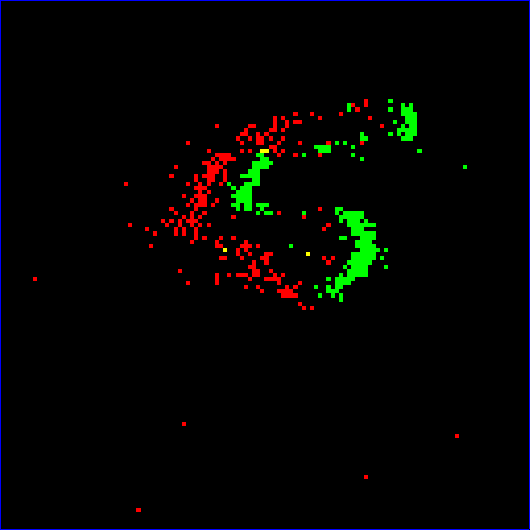
\includegraphics[width=\textwidth]{dvs_demo}
    \caption{Recording from \\silicon retina~\cite{bernabeDVS}.}
    \label{fig:dvs_demo}
  \end{subfigure}
  
  \caption{Visual comparison of an MNIST digit traversing a computer screen horizontally.}
  \label{fig:dvs_vs_cam}
  
\end{figure}

Using conventional cameras, and thus our emulator, enforces certain limitations which we summarize in Table~\ref{tb:constraints}.
\begin{table}
  \centering
  \caption{Emulator limitations.}
  \label{tb:constraints}
  \begin{tabular}{l c c}
    & DVS & Camera (PS3 Eye) \\ 
    \hline
    \rule{0pt}{0.4cm}Power consumption & 24 mW & \~120mW\\
    Response time & 3.6 $\rightarrow$ 15us & 8ms $\rightarrow$ 16ms \\
    Dynamic range & 120 dB & 60 dB\\
  \end{tabular}
\end{table}


The emulator can encode video (live or pre-recorded) and we provide a ``virtual camera'' that simulates movement on images so they can also be perceived. Using the virtual camera and the MNIST hand-written digits database~\cite{mnist,mnist:web} we demonstrate the emulator's extensions. To test encodings we converted an MNIST  digit image which we scaled down to $8\times8$ pixels for clarity and the reference frame's values were initialized at half the scale range, Figure~\ref{fig:spike_codes} shows the spike representation using the developed output encodings.

\setcounter{figure}{12} % -------------- fix figure numbers ----------------- %
\begin{figure*}[htb]
  \captionsetup[subfigure]{justification=centering}
  
  \centering
  \begin{subfigure}[b]{0.3\textwidth}
    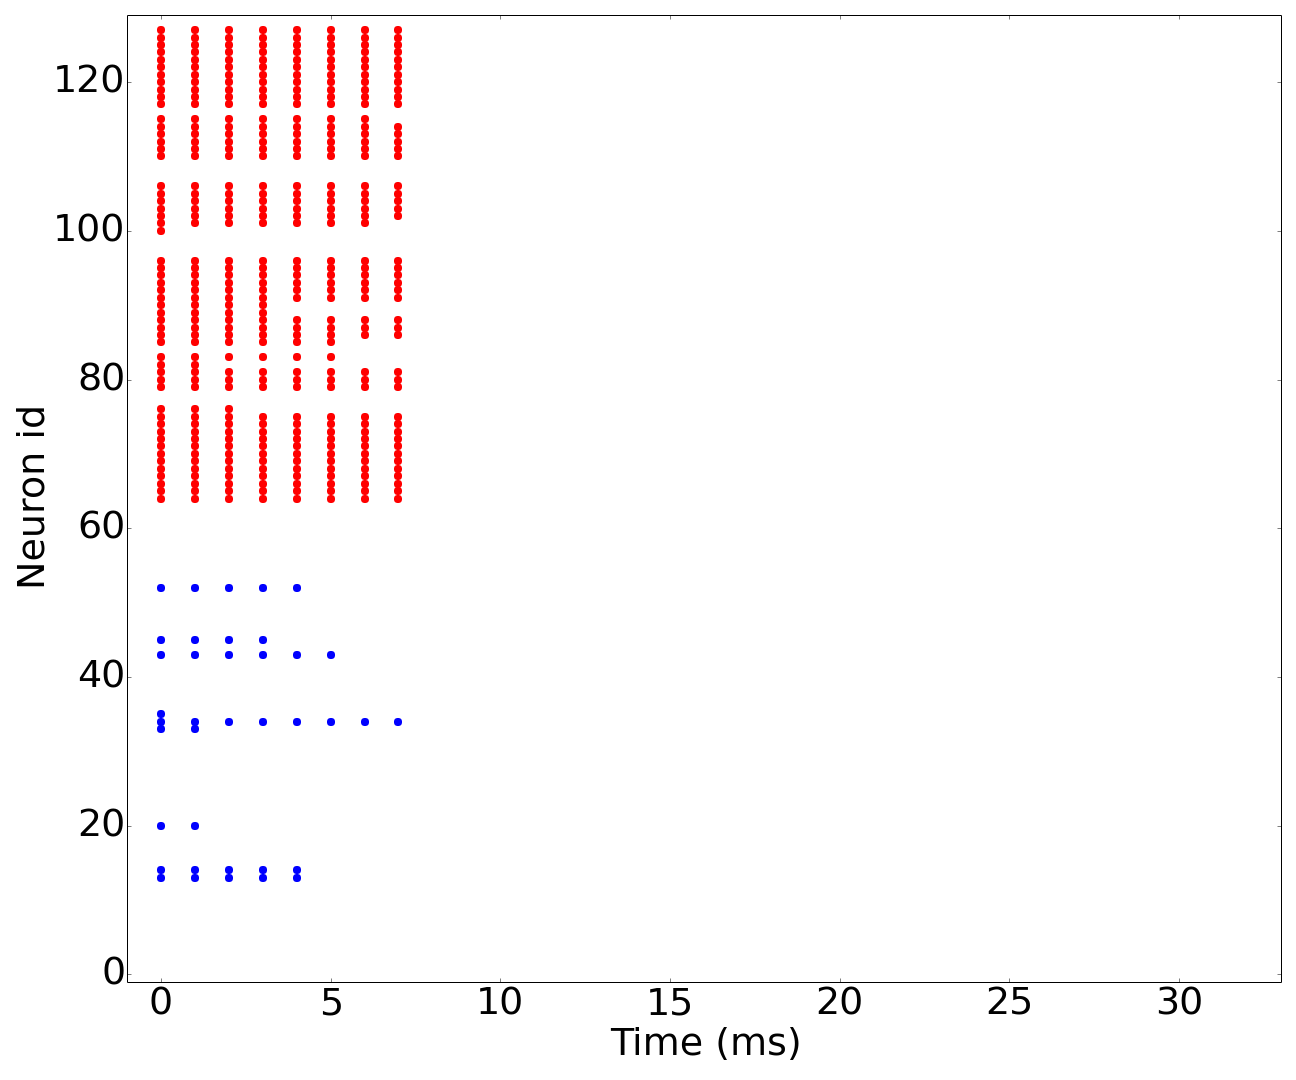
\includegraphics[width=\textwidth]{rate_coded_-8x8-_cycle_0}
    \caption{Rate coded spikes.\\~ }
    \label{fig:rate_spikes}
  \end{subfigure}~
  \begin{subfigure}[b]{0.3\textwidth}
    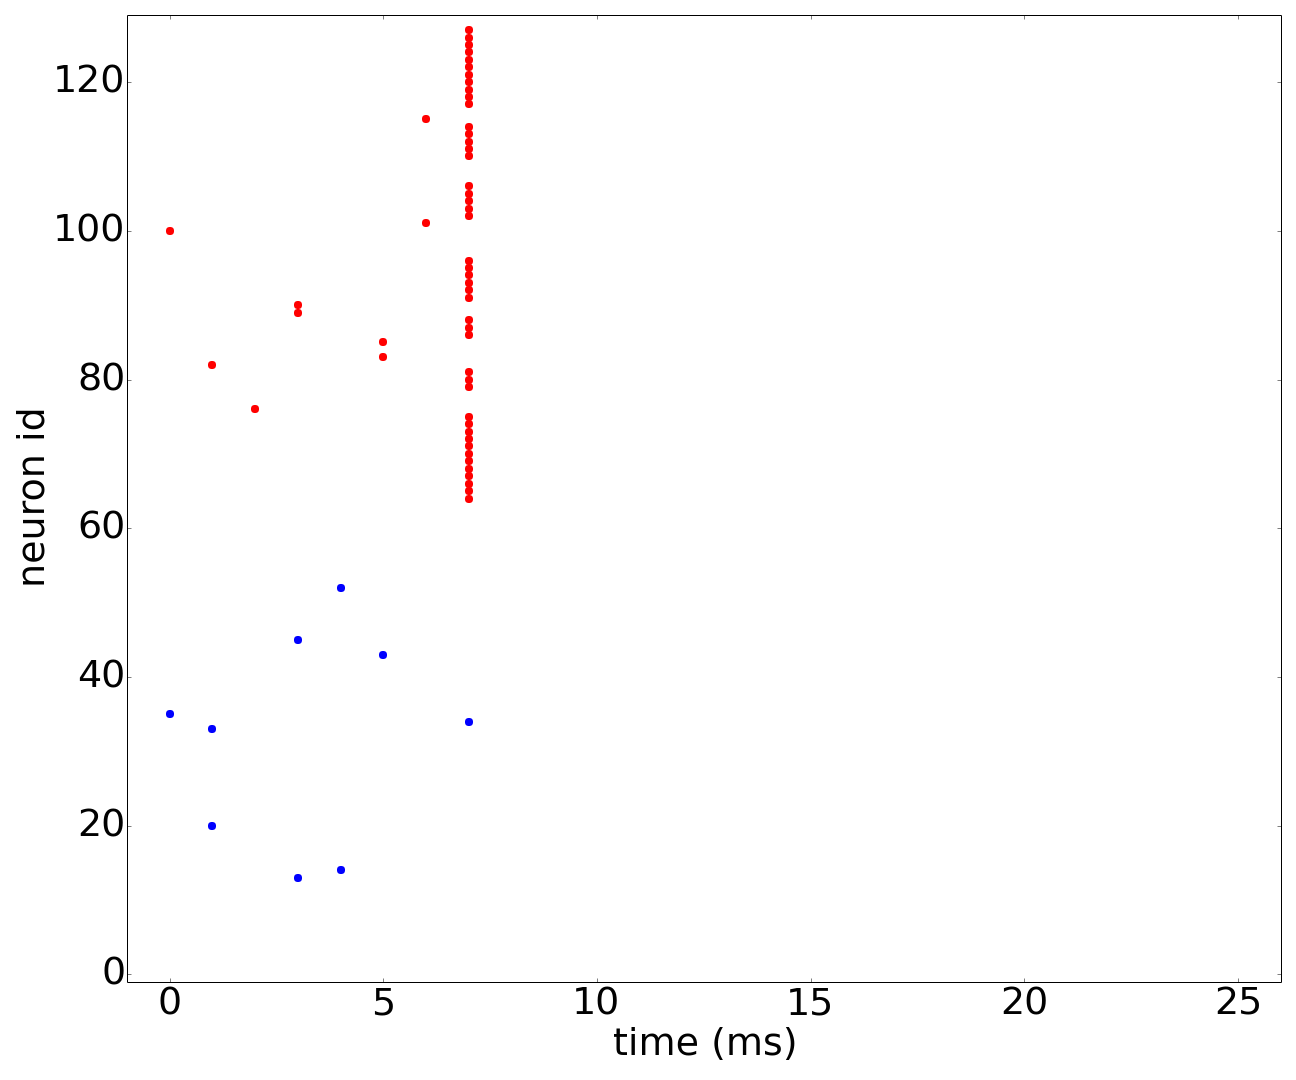
\includegraphics[width=\textwidth]{time_coded_-8x8-_cycle_0}
    \caption{Time coded spikes (linear).\\~}
    \label{fig:time_spikes}
  \end{subfigure}~
  \begin{subfigure}[b]{0.3\textwidth}
    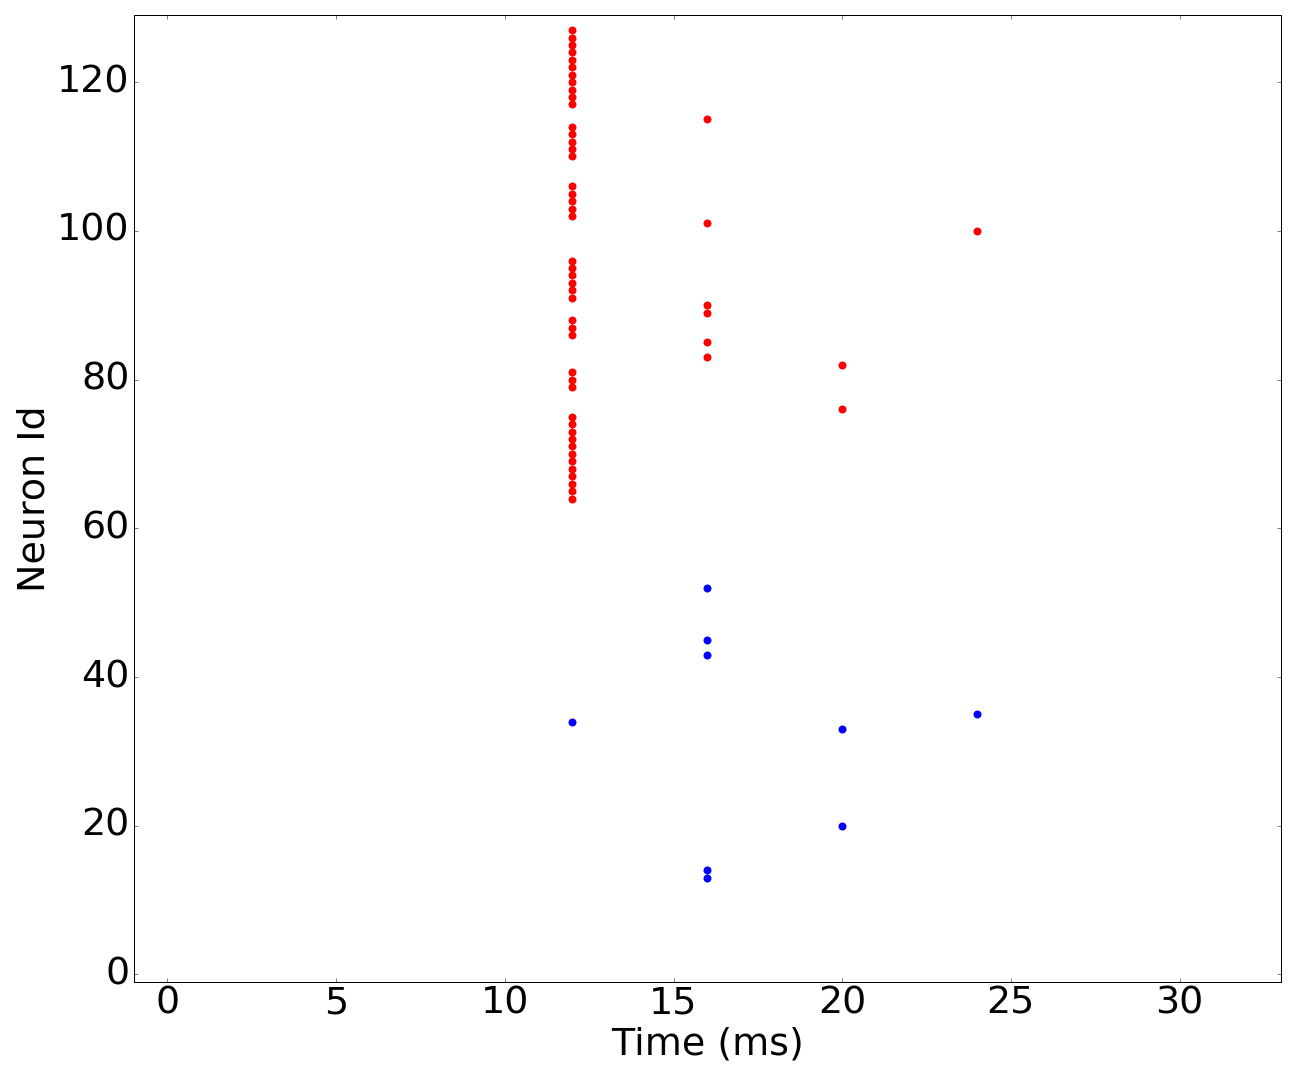
\includegraphics[width=\textwidth]{time_exp_coded_-8x8-_cycle_0}
    \caption{Time coded spikes \\(logarithmic).}
    \label{fig:time_exp_spikes}
  \end{subfigure}
  
  \caption{Difference between spike encodings for the first wave of spikes after the presentation of an MNIST digit.}
  \label{fig:spike_codes}
\end{figure*}


The inhibitory behaviour will reduce the number of spikes that the emulator produces per frame, while keeping some of the information needed to represent the visual input. Figure~\ref{fig:pre_inh} shows the detected spikes as the digit traverses to the right. After the inhibition step fewer spikes remain while keeping the overall shape~(Fig.~\ref{fig:post_inh}). Since not all the information is sent on the first frame and objects in video generally do not move fast enough to disappear between frames, there is a \textit{persistence of vision}-like effect of spikes for succeeding frames. To asses this we removed the spikes that would be generated in the current frame without inhibition (Fig.~\ref{fig:pre_inh}) from the inhibited spike generation (Fig.~\ref{fig:post_inh}), the result (Fig.~\ref{fig:diff_post_inh}) shows spikes that are the result of inhibition in previous frames. This shows a figure that's quite similar to the what we should have detected in preceding frames.

\setcounter{figure}{11} % -------------- fix figure numbers ----------------- %
\begin{figure}[htb]
  \captionsetup[subfigure]{justification=centering}
  \centering
  \begin{subfigure}[b]{0.155\textwidth}
    
\includegraphics[width=\textwidth,trim={3cm 2cm 2cm 2cm},clip] {inhibitory_behaviour__NORMAL___cycle_00000___frame_00035_}
    \caption{Raw spikes.\\~}
    \label{fig:pre_inh}
  \end{subfigure}
  \begin{subfigure}[b]{0.155\textwidth}
    
\includegraphics[width=\textwidth,trim={3cm 2cm 2cm 2cm},clip] {inhibitory_behaviour__INHIBITED___cycle_00000___frame_00035_}
    \caption{Inhibited spikes.\\~}
    \label{fig:post_inh}
  \end{subfigure}
  \begin{subfigure}[b]{0.155\textwidth}
    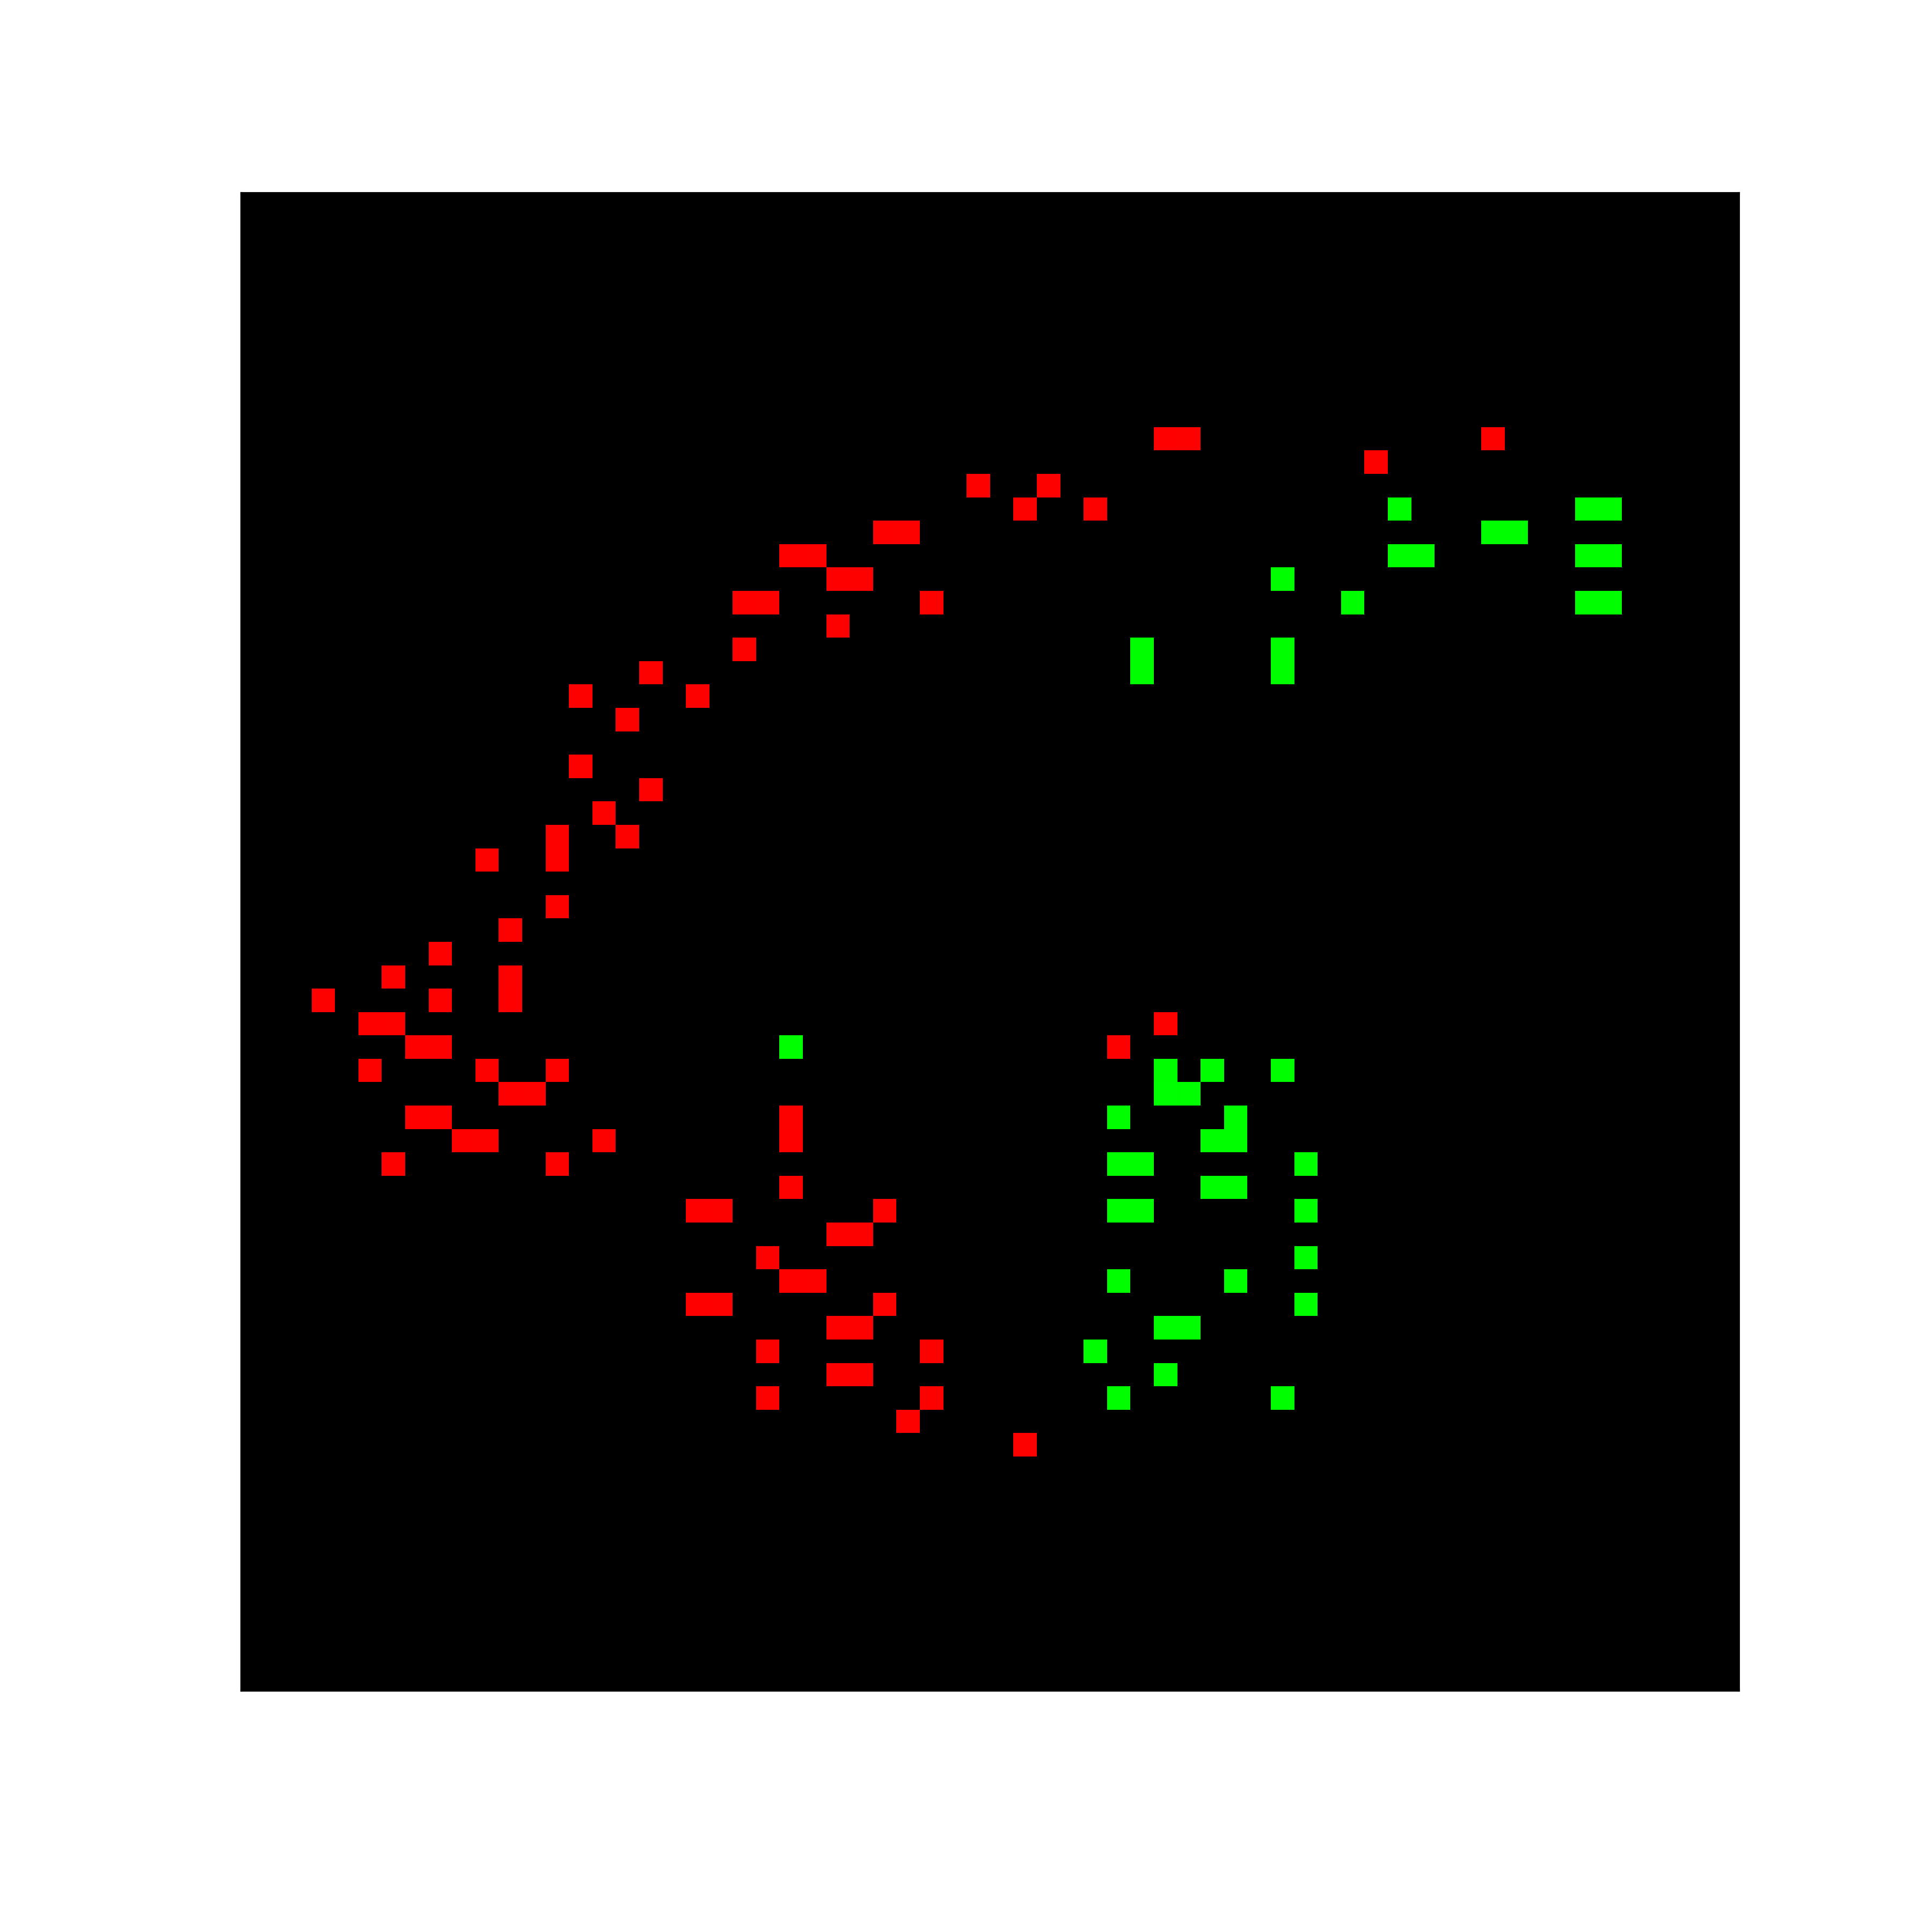
\includegraphics[width=\textwidth,trim={3cm 2cm 2cm 2cm},clip] {inhibitory_behaviour__DIFF___cycle_00000___frame_00035_}
    \caption{Spikes from previous frames.}
    \label{fig:diff_post_inh}
  \end{subfigure}
  \caption[Difference between raw and local inhibited spikes from a traversing image.]{Difference between raw and local inhibited spikes from a traversing image.}
  \label{fig:inh_diff}
\end{figure}
%%%%%%%%%%%%%%
%\footnotetext{Notice that most images in the tests are shown inverted. They originally where white over black and are now altered to black over white to better capture the behaviour}
%%%%%%%%%%%%%%

Finally, we tested the weight decay mechanism, an example of how the receiver can recover from a loss of spikes is shown in Figure~\ref{fig:history_decay}; of particular interest are the $sender$ and $receiver$ rows, which show their respective reference frames (i.e. what both ``see''). The leftmost column illustrates how the system starts and what spikes are going to be sent (``spikes'' row).

If some of the spikes are lost (second column), the receiver cannot reconstruct the picture correctly. After 40 waves of spikes (rightmost column),  pixels in the absolute difference between the reference images ($|send-recv|$ row) have an 8.6 average value which is bellow the threshold. This means that the missing information has been retransmitted due to history decay. Another effect of this mechanism is that the need to constantly move the image is removed since the reference values are continuously lowered; this effect furthers the difference between the image and the reference up to a point at which spikes are produced.

\setcounter{figure}{13} % -------------- fix figure numbers ----------------- %
\begin{figure}[htb]
%  \captionsetup[subfigure]{justification=centering}
  \centering
  
  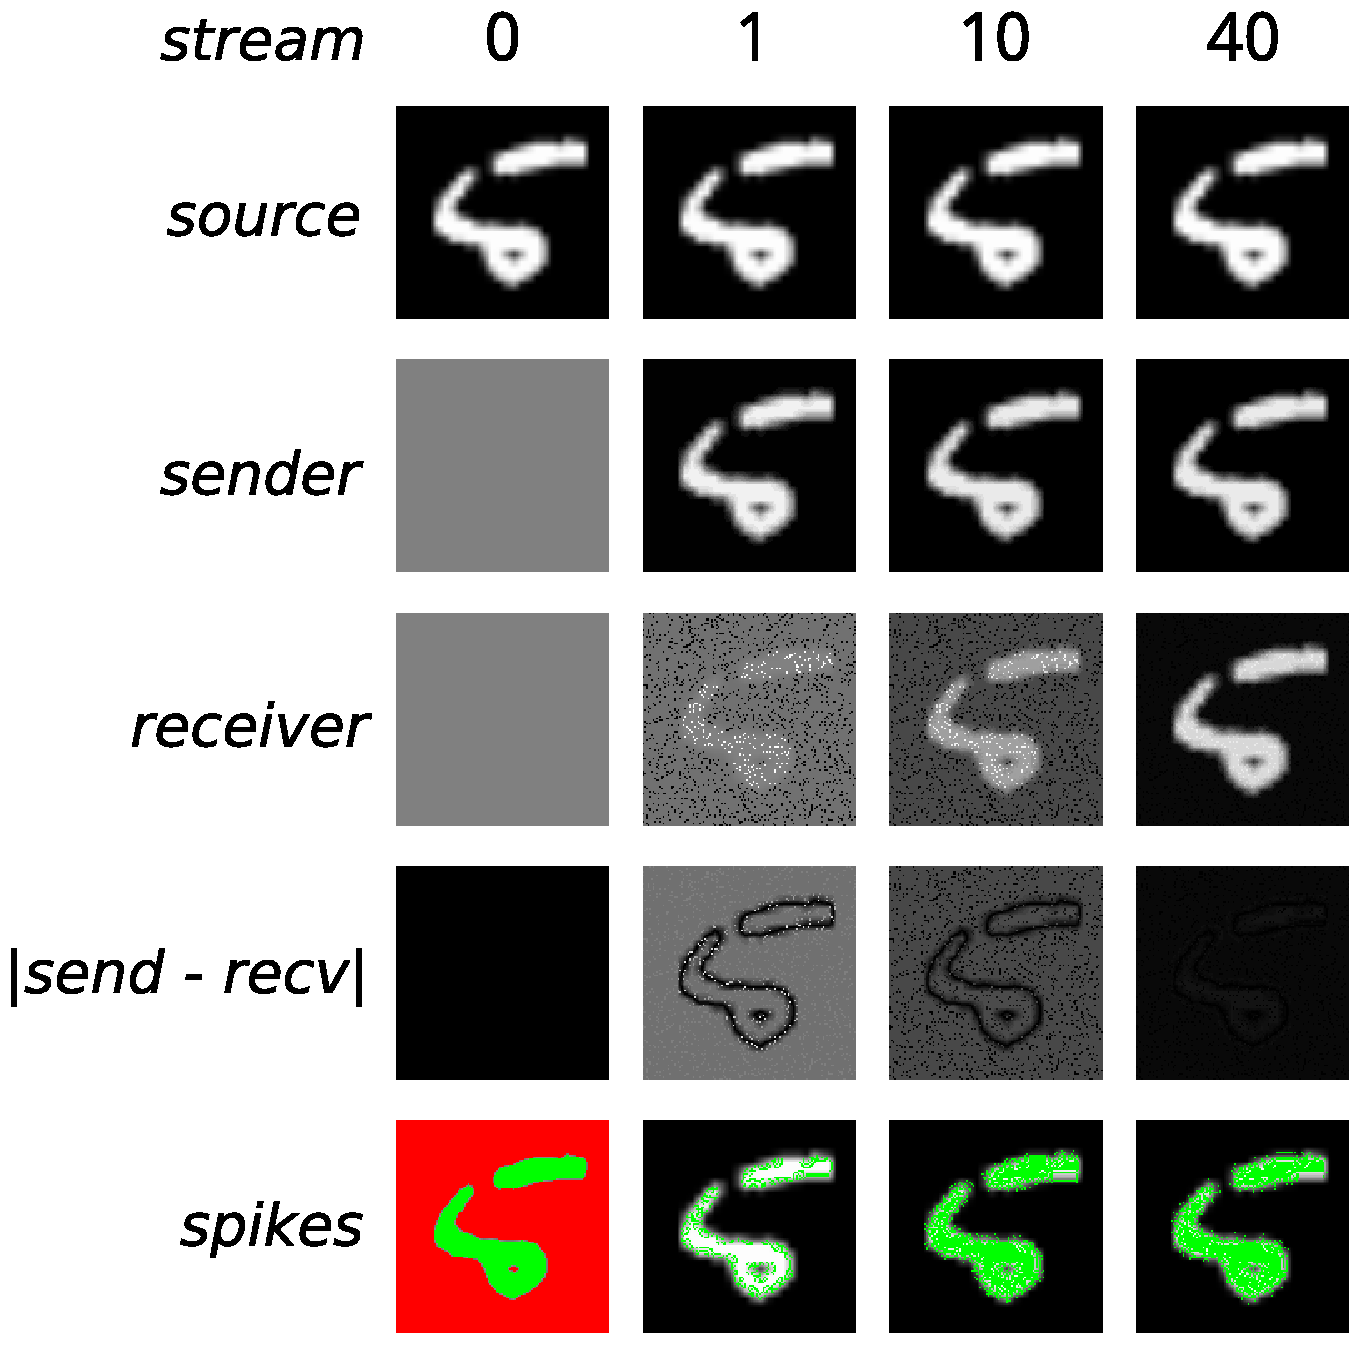
\includegraphics[width=0.45\textwidth]{history_decay}
  \caption{History decay helps to remove transmission errors (1~spike-per-pixel with linear spike-time encoding).}
  \label{fig:history_decay}
\end{figure}


\section{Conclusion}
\label{sec:conclusions}
An important contribution to the field of computer vision research has been the development of image and video databases. To utilize them in spiking neural networks without pointing a DVS at a monitor, we developed the emulator presented here. To encode images we developed a ``virtual camera'' that simulates movement so the pictures can be captured by the DVS. Two of these motions are inspired by eye movements known as saccades.
%Using well known datasets, allows an easier comparison between spiking and traditional neural networks.

Emulating a DVS provides the flexibility to modify the system's behaviour in software. One such change is to encode values represented by spikes using time instead of rate. This allows more information to be sent per spike and lowers bandwidth requirements. 
%mage analysis with time-coded spikes has not been as popular as rate-coded ones, this emulator.

Our inhibitory component splits spike emission into, at most, four frames and it also presents a side-effect similar to persistence of stimuli. If the adaptive threshold block is used, the emulator should filter out fast changing pixels thus reducing the number of spikes emitted. After considering that not all spikes will arrive to their destination, we developed a history decay mechanism for the reference update. This has the effect of fixing transmission errors and continuously sending spikes if pixels' difference of brightness values are larger than the threshold, even without moving images.
%We theorize that it could help to ease timing issues with time-coded spiking networks.

\section{Future work}
\label{sec:future-work}
While the image resolution of the current version of our emulator is low, an OpenCL version has been developed. By using the parallel processing nature of Graphics Processing Units it was possible to encode images at higher resolutions (we have tested up to $1920\times1080$ video at 30 FPS); the main problem with this large imagery is that serializing and transmitting such numbers of spikes has proven a hard task.

Research on encoding spikes using convolution kernels is ongoing. We have explored, using a kernel based on Carver Mead's original silicon retina connectivity~\cite{Mead1989} and biologically inspired difference of Gaussian kernels~\cite{basab}. These types of encoding could prove to be more efficient since a single spike would represent a region of the image instead of a single pixel.
\section*{Acknowledgement}
%EPSRC??? 
%HBP???
The research leading to these results has received funding from the European Research Council under the European Union's Seventh Framework Programme(FP/2007-2013) / ERC Grant Agreement n. 320689 and from the EU Flagship Human Brain Project (FP7-604102).

Garibaldi Pineda García is funded by a National Council for Science and Technology of Mexico PhD Scholarship.

Patrick Camilleri and Steve Furber are supported by EPRSC project EP/K034448/1 (PRiME). 

The authors would like to thank the reviewers for taking the time to review this document and provide useful feedback on the work. They would also like to thank Jim Garside and Viv Woods for help and useful discussions during the course of this paper.

%The authors would like to thank John Viv Woods and Jim Garside for proofreading 
%This work was inspired by talks at the Capo Caccia Workshop.

\bibliography{biblio_dvs_emu_paper}
\bibliographystyle{IEEEtranN}
%\printbibliography


\begin{IEEEbiography}{Garibaldi~Pineda~García}
  Biography text here.
\end{IEEEbiography}
%\end{multicols}
\end{document}
